\documentclass[a4paper, 9pt]{beamer}
\usepackage[T2A]{fontenc}
\usepackage[english,russian]{babel}

% \graphicspath{{images/}}

\usepackage{csquotes, xcolor}
\usepackage{booktabs}
\usepackage[customcolors,shade]{hf-tikz}
\definecolor{mLightBlue}{HTML}{4D59F6}
\definecolor{pGray}{HTML}{949ea0}
\definecolor{pGreen}{HTML}{008000}

\usetheme{metropolis} 

\addto\captionsrussian{ 
\def\figurename{Рисунок} 
}

\usepackage[%
backend=biber,% движок
bibencoding=utf8,% кодировка bib файла
sorting=none,% настройка сортировки списка литературы
maxbibnames=3, % Максимальное число авторов в списке литературы.
minbibnames=3,
style=gost-numeric,% стиль цитирования и библиографии (по ГОСТ)
language=english,% получение языка из babel/polyglossia
autolang=other,% 
clearlang=true,% 
defernumbers=true,% 
sortcites=true,% 
]{biblatex}
\addbibresource{../../TeX/biblio/literature.bib}
\NewBibliographyString{langjapanese}
\NewBibliographyString{fromjapanese}
%\newcommand{\itemi}{\item[\checkmark]}

%\newtotcounter{citenum}
\makeatletter

\defbibenvironment{counter}
  {\setcounter{citenum}{0}
  \renewcommand{\blx@driver}[1]{}
  }
  {} %\thecitenum сюда писать не надо
  {\stepcounter{citenum}}

\@addtoreset{figure}{framenumber}
\@addtoreset{equation}{framenumber}
% \setcounter{subfigure}{0}
\makeatother
\defbibheading{counter}{}

\DeclareSourcemap{
    \maps{
        \map[overwrite]{% стираем значения всех полей issn
            \step[fieldset=doi, null]
        }
        \map[overwrite]{% стираем значения всех полей issn
            \step[fieldset=issn, null]
        }
    }
}

\newcommand\invisiblesection[1]{%
  \refstepcounter{section}%
  \addcontentsline{toc}{section}{\protect\numberline{\thesection}#1}%
  \sectionmark{#1}}

\usepackage{tikz}
\usetikzlibrary{arrows,shapes.geometric,calc,chains}
\usepackage{caption}
\captionsetup[figure]{labelfont={bf},name={\footnotesize Рисунок},labelsep=endash}%period}
\captionsetup[table]{labelfont={bf},name={\footnotesize Таблица},labelsep=endash}%period}

\newcommand{\mycirc}[1]{\tikz{\path[draw=black,fill=#1,line width=0.25] (0,0) circle [radius=0.09];}} % --(0.525,0.25)--(0,0.5)--cycle;}}
\newcommand{\myrec}[1]{\tikz{\path[draw=black,fill=#1,line width=0.25] (0,0) rectangle (0.12,0.20);}} % --(0.525,0.25)--(0,0.5)--cycle;}}

\usetikzlibrary{arrows.meta}
\tikzset{
>=stealth',
punkt/.style={
           rectangle,
           rounded corners,
           draw=black, thick,
           text width=6.5em,
           minimum height=2em,
           text centered},
    pil/.style={
           ->,
           thick,
           shorten <=2pt,
           shorten >=2pt,}
double arrow/.style args={#1 colored by #2 and #3}{
    -stealth,line width=#1,#2, % first arrow
    postaction={draw,-stealth,#3,line width=(#1)/3,
                shorten <=(#1)/3,shorten >=2*(#1)/3}, % second arrow
  }
}
\usepackage[export]{adjustbox}

\title{\large Структурно-параметрическая идентификация \\ имплантируемых роторных насосов крови в \\аппаратах вспомогательного кровообращения}%Идентификация и управление\\ имплантируемым роторным насосом крови\\ в аппаратах вспомогательного кровообращения} % Методы и алгоритмы управления работой имплантируемого роторного насоса крови для аппаратов вспомогательного кровообращения}
\author{\vskip-1.0ex 05.13.01 --  Системный анализ, управление и обработка информации \\(технические системы) \\\vskip1.01ex Диссертация на соискание ученой степени кандидата технических наук \\\vskip1.1ex Научный руководитель: д.ф.-м.н., профессор Селищев С. В.}
\date{\vskip2.5ex Москва -- 2018}

%\author{Национальный исследовательский университет \\ <<Московский институт электронной техники>> \vskip1.0ex ПЕТУХОВ Дмитрий Сергеевич \vskip1.0ex 05.13.01 -- Системный анализ, управление и обработка информации \vskip1.0ex Диссертация на соискание учёной степени кандидата технических наук}

\institute{Министерство образования и науки Российской Федерации \\\vskip1.0ex Федеральное государственное автономное образовательное учреждение высшего образования «Национальный исследовательский университет <<Московский институт электронной техники>> \\\vskip4.0ex \textbf{\normalsize Петухов Дмитрий Сергеевич} \vskip2.0ex}

\begin{document}

\maketitle

% ----------------------------------------------------------------------------------------------------------------------------------------------------------------
% ----------------------------------------------------------------------------------------------------------------------------------------------------------------

\begin{frame}{Аппараты вспомогательного кровообращения -- сложная система}

\begin{minipage}[ht]{0.48\textwidth}
\begin{figure}
\center{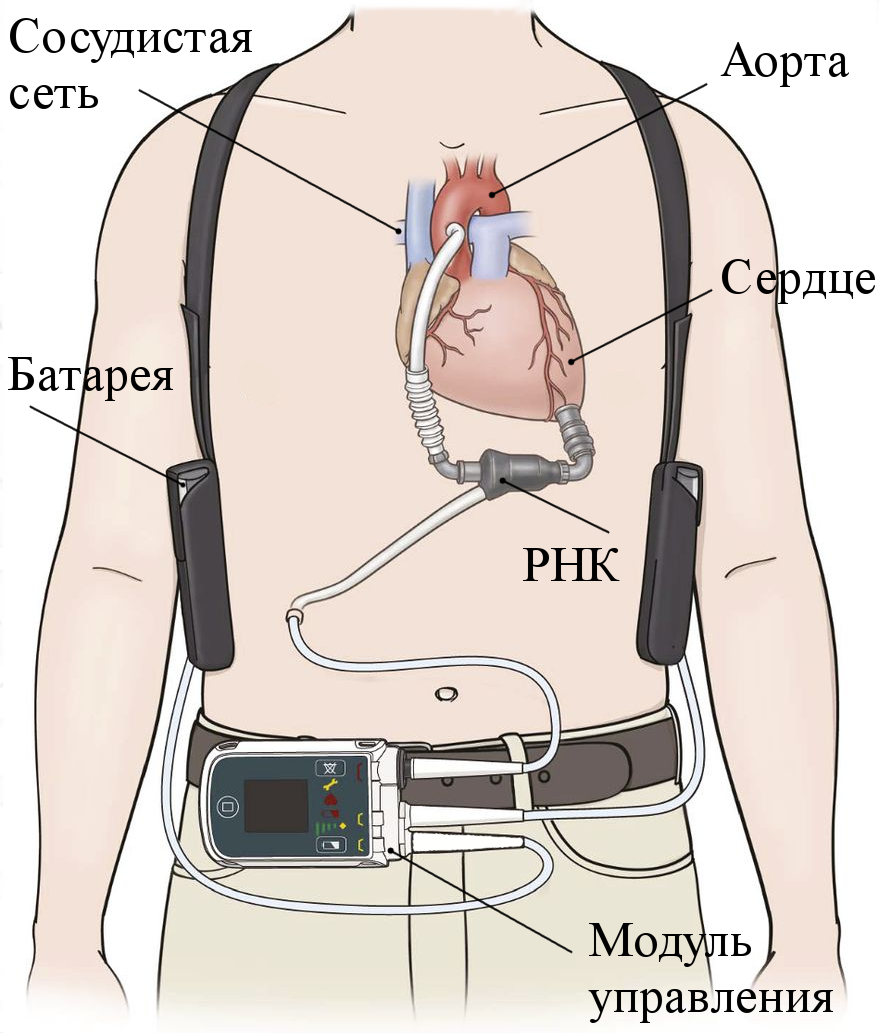
\includegraphics[width=0.72\linewidth]{../images/vad_system}}
\caption{\scriptsize Пример поддержки кровообращения с использованием аппарата вспомогательного кровообращения (АВК); РНК -- роторный насос крови}
\end{figure}
\end{minipage}
\hfill
\begin{minipage}[ht]{0.48\textwidth}
\begin{figure}
\center{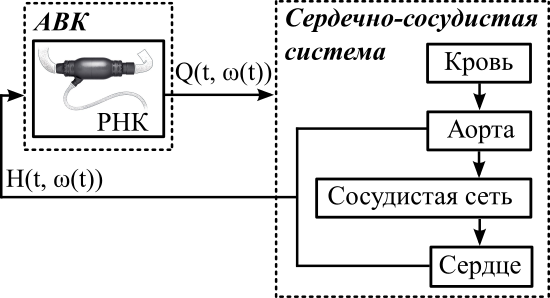
\includegraphics[width=0.95\linewidth]{../images/system_links}}
\caption{\scriptsize Обобщенная схема поддержки кровообращения с помощью АВК; \\ $Q$ -- расход насоса \\$H$ -- перепад давления в насосе \\$\omega$ -- скорость вращения ротора насоса \\$t$ -- время}
\end{figure}
\end{minipage}

\footnotesize
\begin{itemize}
 \item АВК -- сложная техническая система, предназначенная для поддержки кровообращения у пациентов с тяжелой формой сердечной сердечной недостаточности,
 \item С целью управления требуется представление РНК в виде математической модели с определением ее структуры и числовых значений коэффициентов математической модели согласно экспериментальным данным, т. е. \underline{структурно-параметрическая} \underline{идентификация}.
\end{itemize}

\end{frame}

% ----------------------------------------------------------------------------------------------------------------------------------------------------------------
% 
% \begin{frame}{Трасплантация сердца}
% 
% % \begin{minipage}[ht]{0.48\textwidth}
% % \begin{figure}
% % \center{\includegraphics[width=0.90\linewidth]{ht_example_11}}
% % \caption{\small Количество трансплантаций сердца в мире (\footnotesize по данным International Society for Heart and Lung Transplantation -- ISHLT)} % добавить значения индексов
% % \end{figure}
% % \end{minipage}
% % \hfill
% % \begin{minipage}[ht]{0.48\textwidth}
% \begin{figure}
% \center{\includegraphics[width=0.85\linewidth]{ht_trend}}
% \caption{\small Количество трансплантаций сердца в России (\myrec{red}) и США (\myrec{blue}) (\footnotesize по данным Международного регистра органного донорства и трансплантологии -- The International Registry of Organ Donation and Transplantation -- IRODaT) }
% \end{figure}
% %\end{minipage}
% \vskip-10pt
% \begin{figure}
% \center{\includegraphics[width=0.85\linewidth]{vad_trend}}
% \caption{\small Количество имплантаций аппаратов вспомогательного кровообращения (\footnotesize по данным Interagency Registry for Mechanically Assisted Circulatory Support -- INTERMACS) }
% \end{figure}
% 
% \end{frame}

% ----------------------------------------------------------------------------------------------------------------------------------------------------------------

\begin{frame}{Имплантируемые РНК в аппаратах вспомогательного кровообращения}

\begin{minipage}[ht]{0.52\textwidth}
\footnotesize% \emph{Аппараты вспомогательного кровообращения} (АВК) -- альтернатива трансплантации сердца.

%\vskip8pt
Основные элементы АВК:
\begin{itemize}
 \item \alert{Роторный насос крови (РНК)}
 \item Модуль электронного управления
 \item Информационный модуль
 \item Зарядное устройство с батареями
\end{itemize}
\end{minipage}
\hfill
\begin{minipage}[ht]{0.47\textwidth}
%\vskip-10pt
\begin{figure}
 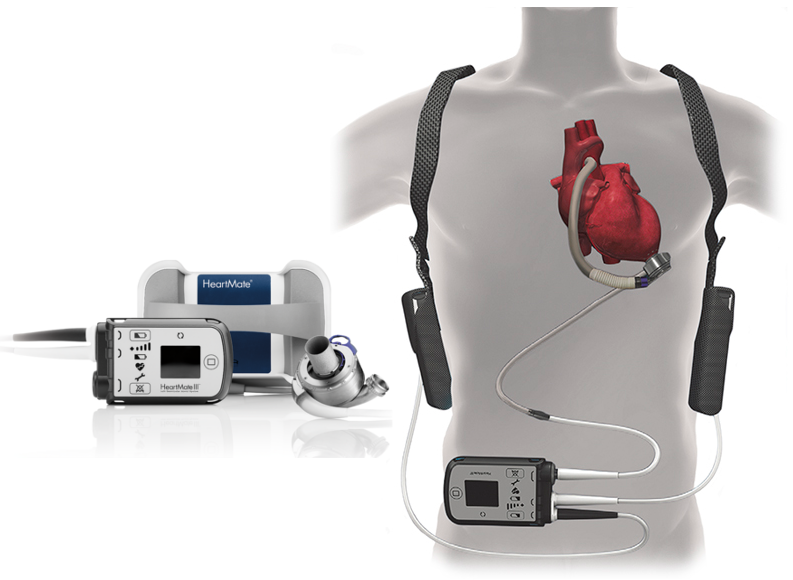
\includegraphics[scale=0.165]{../images/hm_3_pres}
 \caption*{\footnotesize АВК HeartMate 3 (Thoratec Corp., США)} 
\end{figure}
\end{minipage}
\vfill
\begin{minipage}[ht]{.28\textwidth}
\centering

\vskip-14pt
\begin{figure}
  \center
  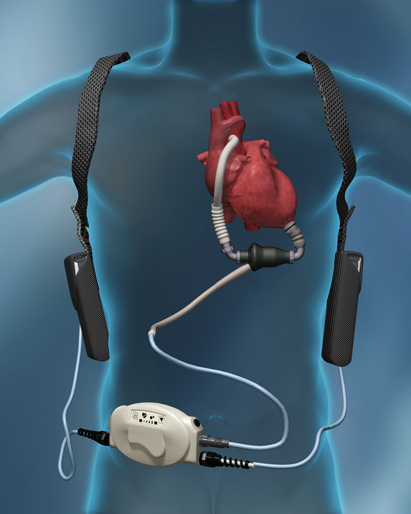
\includegraphics[scale=0.75]{../images/hm_2_pres}
  \caption*{\footnotesize АВК HeartMate 2 (США)} 
\end{figure}

\end{minipage}\hfill
\begin{minipage}[ht]{.36\textwidth}
\centering

\begin{figure}
 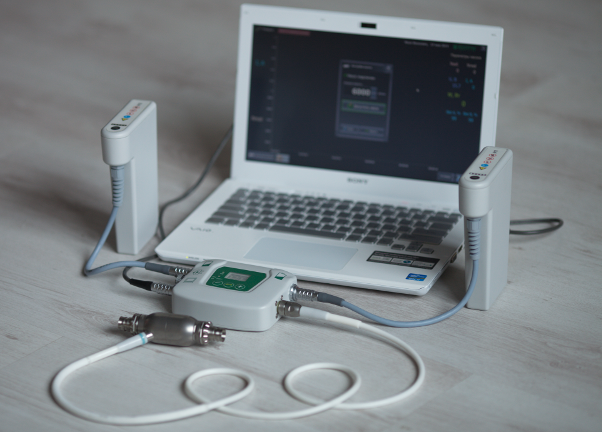
\includegraphics[scale=0.5]{../images/sputnik_pres}
 \caption*{\footnotesize АВК Спутник (Россия)} 
\end{figure}

\end{minipage}\hfill
\begin{minipage}[ht]{.34\textwidth}
\centering \vskip-5pt

\begin{figure}
 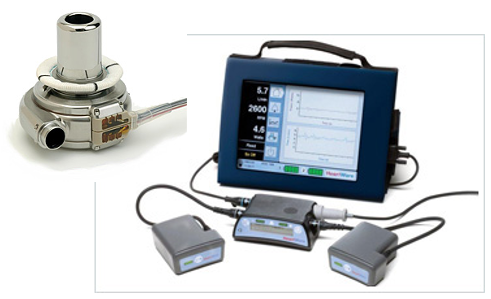
\includegraphics[scale=0.23]{../images/hvad_pres}
 \caption*{\footnotesize АВК HVAD (HeartWare, США)} 
\end{figure}

\end{minipage}

\begin{tikzpicture}[overlay]
\draw[rounded corners, mLightBlue, opacity=0.5, line width=0.75 ] (7.0, 2.25) rectangle (8.65,3.70);
\draw[rounded corners, mLightBlue, opacity=0.6, line width=0.75 ] (3.96, 1.54) rectangle (4.82,2.05);
\draw[rounded corners, mLightBlue, opacity=0.5, line width=0.75 ] (9.2, 6.45) rectangle (10.0,6.85);

\draw[rounded corners, mLightBlue, opacity=0.65, line width=0.75 ] (1.55, 2.45) rectangle (2.22,2.85);

\end{tikzpicture}

\end{frame}

% ----------------------------------------------------------------------------------------------------------------------------------------------------------------

\begin{frame}{Проблема идентификации имплантируемых роторных насосов крови}
\small

\underline{Управление} -- одно из ключевых направлений развития технологии вспомогательного кровообращения \footnotemark[1]$^, $\footnotemark[2], которое: 
\vskip-5pt
\begin{itemize}
 \item \footnotesize нацелено на поддержание достаточного уровня кровообращения в сердечно-сосудистой системе,
 \item должно предотвращать нежелательные состояния в сердечно-сосудистой системе.
\end{itemize}

\footnotesize
\vskip-4pt
Управлению РНК посвящено множество работ российских и зарубежных авторов \footnotemark[1]$^, $\footnotemark[3]. 

\vskip-1pt
Эффективное управление РНК требует точной \underline{идентификации} -- построения математической модели по экспериментальным данным \footnotemark[4].

\vskip-2pt
Проблемы идентификации:
\vskip-6pt
\begin{itemize}
 \item \footnotesize не существует универсального и общепринятого способа идентификации и критериев, по которым оценивается эффективность идентификации для управления РНК \footnotemark[5],
 \begin{itemize}
  \item \footnotesize многообразие имплантируемых роторных насосов крови
  \item РНК -- сложная система \footnotemark[6]
 \end{itemize}
 \item необходимо учитывать взаимодействие имплантируемого РНК с сердечно-сосудистой системой.
\end{itemize}
%работа насоса исследуется без учета либо вязкости жидкости \footnotemark[1], либо инерции жидкости \footnotemark[2], либо не учитываются оба эффекта \footnotemark[3],
% \item направленность на определение только одного состояния в сердечно-сосудистой системе, например, состояния аортального клапана \footnotemark[4],
% \item коллапс желудочка сердца рассматривается как состояние, связанное с разрежением камеры желудочка и определяемое как резкое уменьшение сигналов насоса либо превышение заданного порогового значения \footnotemark[2]$^,$\footnotemark[5],
% \item алгоритмы управления поддерживают производительность насоса в соответствии с потребностями организма, которые не определены \footnotemark[5]$^,$\footnotemark[6].
% \item имплантируемый роторный насос крови в АВК является сложной системой \footnotemark[3], 


\vskip5pt

\footnotetext[1]{\tiny ~\textit{AlOmari A.-H. H., Savkin A. V., Stevens M. et al.} Developments in control systems for rotary left ventricular assist devices for heart failure patients: a review \textcolor{pGray}{// Physiological Measurement. 2013. Vol. 34, no. 1. P. 1--27.} }

\footnotetext[2]{\tiny ~\textit{Petukhov D. S., Telyshev D. V.} Control algorithms for rotary blood pumps used in assisted circulation \textcolor{pGray}{// Biomedical Engineering. 2016. Vol. 50, no. 3. P. 157-160.} }

\footnotetext[3]{\tiny ~\textit{Дозоров К. Н., Иткин Г. П., Адаскин А. В.} Система косвенных измерений для задач управления роторными насосами крови \textcolor{pGray}{// Медицинская техника. 2010. № 6. С. 16-19.} }

\footnotetext[4]{\tiny ~\textit{Гроп Д.} Методы идентификации систем \textcolor{pGray}{Мир, 1979.} }

\footnotetext[5]{\tiny ~\textit{Pirbodaghi T., Weber A., Carrel T., Vandenberghe S.} Effect of Pulsatility on the Mathematical Modeling of Rotary Blood Pumps \textcolor{pGray}{// Artificial Organs. 2011. Vol. 35, no. 8. P. 825-832.} }

%\footnotetext[5]{\tiny ~\textit{Moscato F., Danieli G. A., Schima H.} Dynamic modeling and identification of an axial flow ventricular assist device \textcolor{pGray}{// The International Journal of Artificial Organs. 2009. Vol. 32, no. 6. P. 336-343.} }

\footnotetext[6]{\tiny ~\textit{Bertram C.} Measurement for implantable rotary blood pumps \textcolor{pGray}{// Physiological measurement. 2005. Vol. 26, no. 4. P. 99--117.} }

%\footnotetext[3]{\scriptsize ~\textit{Иткин Г.П., Филатов И.А., Дозоров К.Н., Адаскин А.В.} Косвенные методы определения расхода и напора роторных насосов для крови \textcolor{pGray}{// Вестник трансплантологии и искусственных органов. 2015. Т. 17, С. 97--102.} }

%\footnotetext[4]{\scriptsize ~\textit{Rich J. D., Burkhoff D.} HVAD Flow Waveform Morphologies: Theoretical Foundation and Implications for Clinical Practice \textcolor{pGray}{// ASAIO journal. 2017.} }

% \footnotetext[3]{\scriptsize ~\textit{Быков И.В., Иткин Г.П.} Оценка состояния аортального клапана при механической поддержке кровообращения с использованием математической модели \textcolor{pGray}{// Вестник трансплантологии и искусственных органов. 2014. Т. 16, С. 62--67.} }

%\footnotetext[5]{\scriptsize ~\textit{Granegger M, Schima H, Zimpfer D, Moscato F.} Assessment of Aortic Valve Opening During Rotary Blood Pump Support Using Pump Signals \textcolor{pGray}{// Artificial Organs. 2014. Vol. 38, no. 4. P. 290--297.} }

%\footnotetext[6]{\scriptsize ~\textit{Wang Y., Koenig S. C., Slaughter M. S., Giridharan G. A.} Rotary Blood Pump Control Strategy for Preventing Left Ventricular Suction \textcolor{pGray}{// ASAIO Journal. 2015. Vol. 61, no. 1. P. 21--30.} }

%\footnotetext[7]{\scriptsize ~\textit{Дозоров К.Н., Иткин Г.П., Адаскин А.В.} Система косвенных измерений для задач управления роторными насосами крови \textcolor{pGray}{// Медицинская техника. 2010. Т. 6, С. 16--19.} }

\end{frame}

% ----------------------------------------------------------------------------------------------------------------------------------------------------------------
% ----------------------------------------------------------------------------------------------------------------------------------------------------------------

\begin{frame}{Цель и задачи диссертационной работы}
\small
\textbf{Цель}: разработка и исследование способов структурно-параметрической идентификации имплантируемых роторных насосов крови для повышения эффективности идентификации и управления имплантируемыми роторными насосами крови в аппаратах вспомогательного кровообращения.

В~соответствии с целью диссертационной работы поставлены следующие \textbf{задачи}:
\small

\begin{enumerate}
  \item Разработка математической модели идентификации имплантируемого роторного насоса крови на основе расходно-напорных характеристик.
  \item Разработка математической модели сердечно-сосудистой системы с учетом имплантации роторного насоса крови.
  \item Исследование взаимодействия имплантируемого роторного насоса крови и сердечно-сосудистой системы методами математического моделирования и анализ результатов исследования с целью повышения эффективности идентификации и управления имплантируемым роторным насосом крови.
  \item Исследование взаимодействия имплантируемого роторного насоса крови и сердечно-сосудистой системы с использованием экспериментальных данных для роторных насосов крови Спутник с целью верификации результатов математического моделирования.
\end{enumerate}

\end{frame}

\begin{frame}{Положения, выносимые на защиту}
\small

\begin{enumerate}
  \item Предложены критерии, которые позволяют оценить эффективность идентификации для управления имплантируемыми роторными насосами крови в аппаратах вспомогательного кровообращения.
  \item Разработанный алгоритм структурно-параметрической идентификации позволяет построить математические модели имплантируемых роторных насосов крови в соответствии с критериями оценки эффективности идентификации.
  \item Построенные математические модели имплантируемых роторных насосов крови позволяют определить переходы между следующими режимами работы насоса: обратное течение через насос, частичная и полная разгрузка желудочка сердца, и коллапс желудочка сердца.
  \item Разработанный способ управления имплантируемым роторным насосом крови позволяет поддерживать заданный уровень расхода насоса и предотвращать следующие нежелательные режимы работы насоса: обратное течение через насос, полная разгрузка желудочка сердца и коллапс желудочка сердца. 
\end{enumerate}

\end{frame}

% ----------------------------------------------------------------------------------------------------------------------------------------------------------------

\begin{frame}{Разработка модели идентификации имплантируемого РНК}
\scriptsize
\vskip-3pt
Экспериментальные данные -- расходно-напорные характеристики (РНХ) имплантируемого роторного насоса крови HeartMate II \footnotemark[1]$^, $\footnotemark[2]
\vskip-7pt
\begin{minipage}[ht]{0.48\textwidth}
\begin{figure}
\center{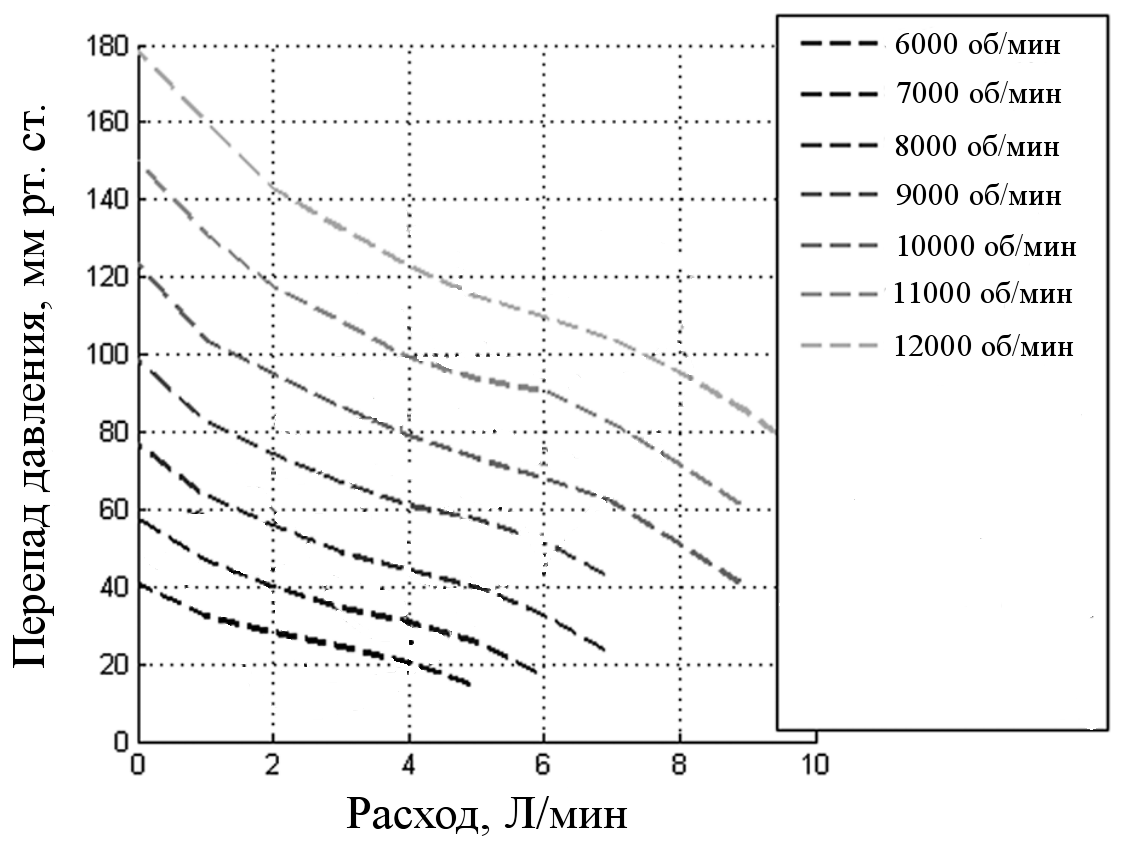
\includegraphics[width=0.55\linewidth]{../images/c2_basic_hq_static}} \vskip-5pt
\caption{\scriptsize РНХ насоса HeartMate II \footnotemark[1]}
\end{figure}
\end{minipage}
\hfill
\begin{minipage}[ht]{0.48\textwidth}
\vskip2pt
\begin{figure}
\center{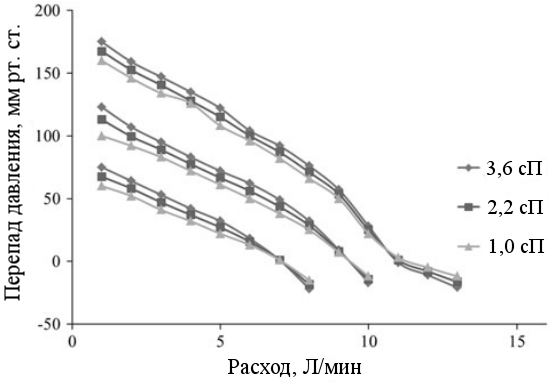
\includegraphics[width=0.55\linewidth]{../images/c2_basic_hq_static_viscosity}} \vskip-5pt
\caption{\scriptsize РНХ насоса HeartMate II при различных величинах вязкости жидкости \footnotemark[2]}
\end{figure}

\end{minipage}
\vskip-11pt
Структура математической модели для описания РНХ согласно работам \footnotemark[3]$^, $\footnotemark[4]:

\vskip-11pt
\begin{equation}
	L\frac{dQ}{dt} = (a_1\mu+a_2)Q + (b_1\mu+b_2)\omega^2 + H,
\end{equation}

\vskip-7pt
\tiny где $L$ -- параметр, характеризующий инерцию жидкости в насосе \footnotemark[4], $Q$ -- расход насоса, $\mu$ -- параметр, характеризующий вязкость жидкости в насосе, $\omega$ -- скорость вращения ротора насоса, $H$ -- перепад давления в насосе, $a$ и $b$ -- коэффициенты.

\vskip-4pt
\scriptsize
\underline{Критерий оценки эффективности идентификации} -- коэффициент детерминации $R^2$:

\vskip-10pt
\begin{equation}
	R^2 = 1- \frac{{\scriptstyle \sum\limits_{i=1}^n} (Q_i - \hat{Q_i})^2}{{\scriptstyle \sum\limits_{i=1}^n} (Q_i - \widetilde{Q_i})^2}, ~~~~\widetilde{Q_i} = \frac{1}{n} \sum\limits_{i=1}^n Q_i
\end{equation}
\vskip-8pt

\tiny 
$R^2$ характеризует долю дисперсии $Q$, объясненную моделью идентификации; чем выше значение $R^2$, тем больше соответствие модели данным и точнее описание объекта управления.

\vskip5pt
\footnotetext[1]{\tiny ~\textit{Pennings K. A., Martina J. R., Rodermans B. F. et al.} Pump Flow Estimation From Pressure Head and Power Uptake for the HeartAssist5, HeartMate II, and HeartWare VADs \textcolor{pGray}{// ASAIO Journal. 2013. Vol. 59, no. 4. P. 420-426.} }
\footnotetext[2]{\tiny ~\textit{Stanfield J., Selzman C.} Pressure Sensitivity of Axial-Flow and Centrifugal-Flow Left Ventricular Assist Devices \textcolor{pGray}{// Cardiovascular Engineering and Technology. 2012. Vol. 3, no. 4. P. 413-423.} }
\footnotetext[3]{\tiny ~\textit{Pirbodaghi T., Weber A., Carrel T., Vandenberghe S.} Effect of Pulsatility on the Mathematical Modeling of Rotary Blood Pumps \textcolor{pGray}{// Artificial Organs. 2011. Vol. 35, no. 8. P. 825-832.} }
\footnotetext[4]{\tiny ~\textit{Moscato F., Danieli G. A., Schima H.} Dynamic modeling and identification of an axial flow ventricular assist device \textcolor{pGray}{// The International Journal of Artificial Organs. 2009. Vol. 32, no. 6. P. 336-343.} }

\end{frame}

% -------------------------------------------------------------------------------

\begin{frame}{Структурно-параметрическая идентификация имплантируемого РНК}
\tiny

\begin{minipage}[ht]{0.35\textwidth} 

\emph{РНХ математических моделей} \\ при различных $R^2$:

\vskip-6pt
\begin{figure}
\center{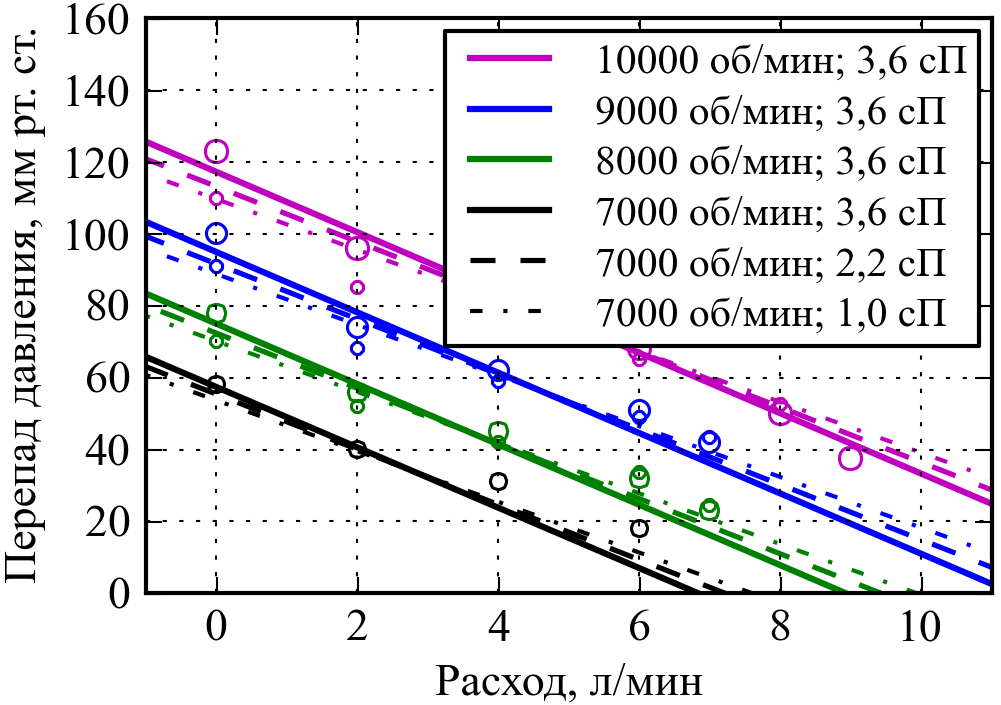
\includegraphics[width=0.75\linewidth]{../images/static_model_initial_pres}}
\vskip-6pt
\caption{\tiny Моделируемые РНХ \\ с $R^2 =$ 0,9566}
\end{figure}

\vskip-12pt
\begin{figure}
\center{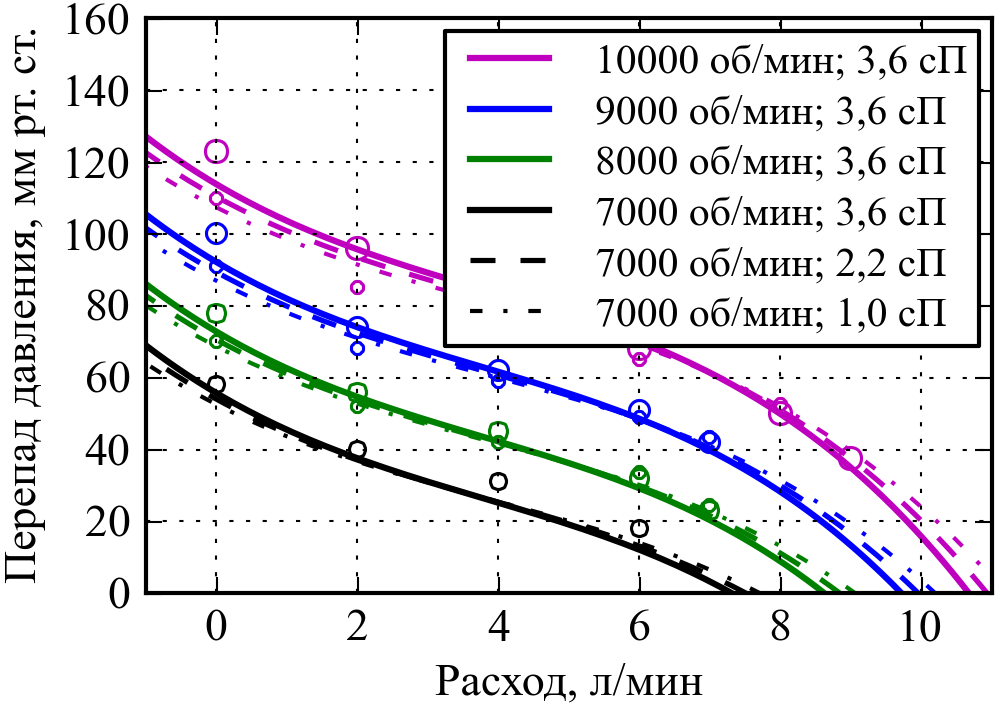
\includegraphics[width=0.75\linewidth]{../images/static_model_updated_pres}}
\vskip-6pt
\caption{\tiny Моделируемые РНХ \\ с $R^2 =$ 0,9738}
\end{figure}

\vskip-12pt
\begin{figure}
\center{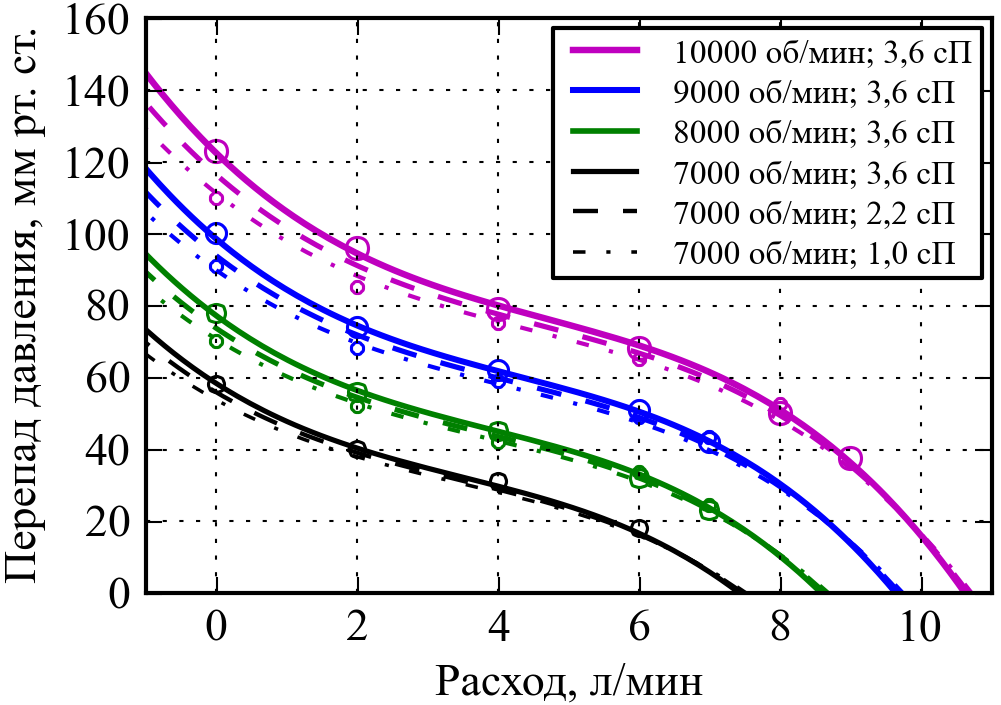
\includegraphics[width=0.75\linewidth]{../images/static_model_final_pres}}
\vskip-6pt
\caption{\tiny Моделируемые РНХ \\ с $R^2 =$ 0,9987}
\end{figure}

\end{minipage}
\hfill
\begin{minipage}[ht]{0.62\textwidth}

\vskip-6pt
\underline{\textbf{Алгоритм структурно-параметрической идентификации}}: \vskip0pt

$R^2 \geq$ 0,9980 -- критерий оценки эффективности идентификации

Структура исходного уравнения:

\vskip-7pt
\begin{equation}
	LdQ/dt =  (a_1\mu+a_2)Q + (b_1\mu+b_2)\omega^2 + H.
\end{equation}

\vskip-5pt
\begin{tikzpicture}[node distance=0.8cm,overlay]
\tikzstyle{startstop} = [rectangle, rounded corners, minimum width=1.2cm, minimum height=0.6cm,text centered, draw=black, fill=gray!10,xshift=2.5cm,yshift=-5.2]
\tikzstyle{io} = [trapezium, trapezium left angle=70, trapezium right angle=110, minimum width=0.9cm, minimum height=0.6cm, text centered, draw=black, fill=gray!10]
\tikzstyle{process} = [rectangle, minimum width=1.1cm, minimum height=0.5cm, text centered, draw=black, fill=blue!30]
\tikzstyle{decision} = [diamond, minimum width=1.5cm, minimum height=0.65cm, text centered, draw=black, fill=gray!10]
\tikzstyle{arrow} = [thick,->,>=stealth]

\node (start) [startstop] {\parbox{2.7cm}{Задание исходного уравнения $y_i$ где $i$ -- номер итерации}};
\node (in1) [io, below of=start, yshift=-3.00] {\parbox{2.5cm}{Добавление к $y_i$ одночлена вида $kx_j$ где $k$ -- коэффициент \\ $j$ -- номер одночлена}};
\node (pro1) [process, below of=in1, yshift=-12.0] {\parbox{3.4cm}{Оптимизация коэффициентов $y_i + kx_j$ с использованием процедуры на основе алгоритма Левенберга-Марквардта \\ Проверка соответствия критерию оценки эффективности идентификации $R^2$}};
\node (dec1) [decision, below of=pro1, yshift=-0.35cm, minimum width=1.8cm] {};% {\footnotesize\bf \parbox{1.5cm}{Соответствие \\ критериям}};
\node (dec2) [decision, below of=dec1, yshift=-0.05cm, minimum width=1.8cm] {};
\node (out2a) [process, right of=dec2, xshift=1.9cm, minimum width=1.0cm, fill=yellow!40] {\parbox{2.2cm}{Задание $y_i + kx_j$ исходным уравнением \\ $i = i + 1$ \\ $j = j + 1$}};
\node (out2b) [process, left of=dec1, xshift=-1.3cm, minimum width=1.0cm, fill=red!40] {\parbox{1.7cm}{Исключение $y_i + kx_j$ \\ $j = j + 1$}};
\node (out2c) [startstop, below of=dec2, xshift=-2.5cm, yshift=0.2cm, minimum height=0.5cm, fill=green!40] {\parbox{2.0cm}{Окончательное $y_i + kx_j$}};
% \node (stop) [startstop, below of=dec1, yshift=-1.1cm, fill=green!40, yshift=-0.1cm] {\small Окончательное $y_i + kx_j$};

\draw [arrow] (start) -- (in1);
\draw [arrow] (in1) -- (pro1);
\draw [arrow] (pro1) -- (dec1);
\draw [arrow] (dec2) -- node[anchor=south] {нет} (out2a);
\draw [arrow] (dec1) -- node[anchor=south] {~~~~~~нет} (out2b);
\draw [arrow] (dec1) -- node[anchor=west] {~~да} (dec2);
\draw [arrow] (dec2) -- node[anchor=west] {~~да} (out2c);
\draw [arrow] (out2a) |- ($(in1.east)+(0,-0.1)$);
\draw [arrow] (out2b) |- ($(in1.west)+(0.05,0.1)$);
%\draw [arrow] (out2b) ($(out2b.east)$)|- + (2.5,0) |- ($(in1.east)+(0.05,0.1)$); 
\draw (2.5, -3.50) node {$R^2_{ij} > R^2_i$}; %  \\ $\delta(PS) \geq 85\%$
\draw (2.5, -4.35) node {$R^2_{ij} \geq 0,9980$}; %  \\ $\delta(PS) \geq 85\%$
\end{tikzpicture}

\vskip152pt

Следующий этап идентификации -- добавление членов $Q^2$ и $Q^3$, что позволило увеличить $R^2$ до 0,9700 и моделировать $S$-образный изгиб РНХ -- рисунок 2:

\vskip-5pt
\begin{equation}
	\setcounter{equation}{2}
	L\frac{dQ}{dt} = aQ + b\omega^2 + cQ^2 + dQ^3 - H,
\end{equation}

\vskip-4pt
где $a-d$ -- коэффициенты, представленные функцией вида $x(\mu) = x_1\mu + x_2$.

В результате математическая модель идентификации описывается уравнением:

\vskip-2pt
% \begin{equation*}
% 	L\frac{dQ}{dt} = aQ + b\omega^2 +~ \tikzmarkin[set fill color=blue!10,set border color=blue!70]{b}(0.095,-0.2)(-0.095,0.4) cQ^2 + dQ^3 \tikzmarkend{b} ~+~ \tikzmarkin[set fill color=red!10,set border color=red!70]{c}(0.095,-0.2)(-0.095,0.4) eQ\omega^2 + fQ^2\omega\tikzmarkend{c} ~+ g - H,
% \end{equation*}
\vskip-3pt
\begin{equation}
	\setcounter{equation}{3}
	L\frac{dQ}{dt} = aQ + b\omega^2 + cQ^2 + dQ^3 + eQ\omega^2 + fQ^2\omega + g - H.
\end{equation}

% \vskip-4pt
% где $L$ -- параметр, характеризующий инерцию жидкости в насосе, $Q$ -- расход насоса, $\omega$ -- скорость вращения ротора насоса (об/мин), $H$ -- перепад давления в насосе, $\mu$ -- параметр, характеризующий вязкость жидкости, $a-g$ -- коэффициенты уравнения, представленные функцией вида $x = x_1\mu + x2$.

% \vskip-4pt
% \begin{itemize}
%  \item члены вида ${\color{blue}Q^2}$ и ${\color{blue}Q^3}$ позволяют воспроизвести $S$-образную форму РНХ,% характерной для 
% \end{itemize}
% \vskip-8pt
% \begin{itemize}
%  \item члены вида ${\color{red}Q\omega^2}$ и ${\color{red}Q^2 \omega}$ позволяют воспроизвести влияние вязкости жидкости на наклон РНХ. % 
% \end{itemize}

% \vskip-2pt
% \begin{itemize}
%  \item члены вида ${\color{blue}Q^2}$ и ${\color{blue}Q^3}$ позволяют воспроизвести $S$-образную форму расходно-напорной кривой,% характерной для 
%  \item члены вида ${\color{red}Q\omega^2}$ и ${\color{red}Q^2 \omega}$ позволяют воспроизвести влияние вязкости жидкости на наклон РНХ, \vskip-5pt % 
%  %\item коэффициенты $a-g$ представлены линейной функцией вида $y(\mu) = k\mu + x$ где $\mu$ -- вязкость (сП),
%  %\item $g$ -- поправочный коэффициент.
%  \item значения коэффициентов уравнения рассчитаны с помощью разработанной процедуры оптимизации на основе алгоритма Левенберга-Марквардта.
% \end{itemize}


\end{minipage}

\end{frame}

% ------------------------------------------------------------------------------

\begin{frame}{Режимы работы имплантируемого РНК}

\footnotesize %\vskip-25pt
Режимы работы РНК -- состояния в сердечно-сосудистой системе, обусловленные спецификой работы РНК \footnotemark[1].% \footfullcite{Karantonis_2006}:

Предотвращение нежелательных режимов работы насоса является одной из основных задач при управлении РНК \footnotemark[2]$^-$\footnotemark[4], для эффективного решения которой необходима точная идентификация.

\vskip10pt
\begin{minipage}[bht]{0.20\textwidth}
\begin{figure}
	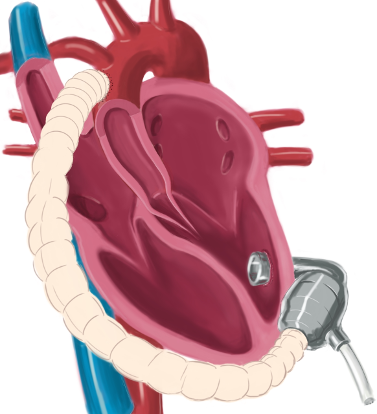
\includegraphics[width=0.85\textwidth]{../images/heart_ps_pres}
	\caption*{\scriptsize Режим обратного течения через насос $\bf P_{BF}$}
\end{figure}
\end{minipage}
\hfill
\begin{minipage}[bht]{0.22\textwidth}
\begin{figure}
	\vskip5pt
	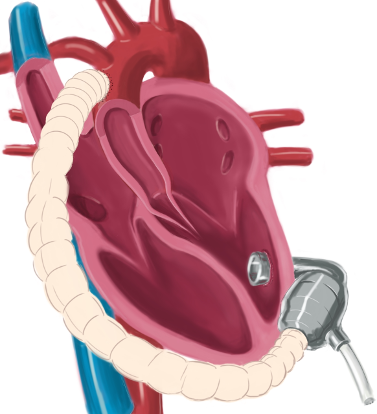
\includegraphics[width=0.85\textwidth]{../images/heart_ps_pres}
	\caption*{\scriptsize Режим частичной разгрузки левого желудочка сердца \\ $\bf P_{PA}$}
\end{figure}
\end{minipage}
\hfill
\begin{minipage}[bht]{0.24\textwidth}
\begin{figure}
	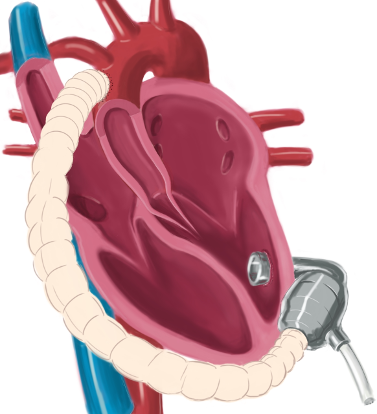
\includegraphics[width=0.85\textwidth]{../images/heart_ps_pres}
	\caption*{\scriptsize Режим полной разгрузки левого желудочка сердца $\bf P_{FA}$}
\end{figure}
\end{minipage}
\hfill
\begin{minipage}[bht]{0.26\textwidth}
\begin{figure}
	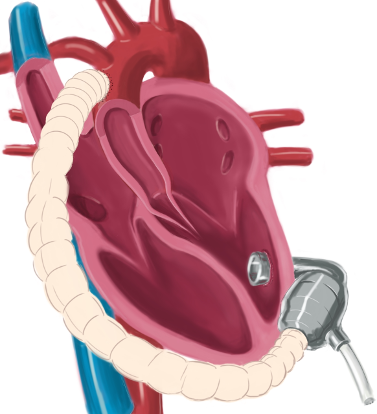
\includegraphics[width=0.85\textwidth]{../images/heart_ps_pres}
	\caption*{\scriptsize Режим коллапса левого желудочка сердца $\bf P_{VC}$}
\end{figure}
\end{minipage}

\footnotetext[1]{\tiny ~\textit{Karantonis D. M., Lovell N. H., Ayre P. J. et al.} Identification and Classification of Physiologically Significant Pumping States in an Implantable Rotary Blood Pump \textcolor{pGray}{// Artificial Organs. 2006. Vol. 30, no. 9. P. 671-679.} }

\footnotetext[2]{\tiny ~\textit{Petukhov D. S., Telyshev D. V., Selishchev S. V.} Control method of a rotary blood pump for a left ventricular assist device \textcolor{pGray}{// Sovremennye tehnologii v medicine 2016. Vol. 8, no. 1. P. 28-33.}}

\footnotetext[3]{\tiny ~\textit{Petukhov D. S., Telyshev D. V.} Control strategy for an implantable rotary blood pump based on identification of pumping states \textcolor{pGray}{// 61st ASAIO Annual Conference. 2015. P. 4.}}

\footnotetext[4]{\tiny ~\textit{Petukhov D. S., Telyshev D. V.} Design concept of patient-adaptive control method for a ventricular assist device \textcolor{pGray}{// 37th Annual International Conference of the IEEE Engineering in Medicine and Biology Society. 2015. P. 116.}}

\begin{tikzpicture}[overlay]
    \draw (1.80, 1.80) node {$Q_{Pump}$};
	\path[-stealth, color=red, line width=1.0] (1.40,1.80) edge [bend left=40] (0.15,2.7);
	\path[-stealth, color=blue, line width=1.0] (0.70,2.25) edge [bend right=25] (1.55,2.10);

    %\draw (3, -1.95) node {$Q_{Pump}$};
    %\draw (1.75, 0.15) node {$Q_{AV}$};
	%\path[-stealth, color=red, line width=1.0] (3.8,-2.0) edge [bend left=50] (0.8,-0.7);
	\path[-stealth, color=red, line width=1.1] (3.85,2.75) edge [bend left=15] (3.4,3.2);
	%\path[-stealth, color=red, line width=1.0] (9.8,1.75) edge [bend left=40] (8.45,2.7);

    %\draw (3, -1.95) node {$Q_{Pump}$};
    \draw (4.35,3.0) node {$Q_{AV}$};
	%\path[-stealth, color=red, line width=1.0] (3.8,-2.0) edge [bend left=50] (0.8,-0.7);
	\path[-, color=red, line width=1.1] (6.5,2.75) edge [bend left=0] (6.1,3.2);
	\path[-, color=red, line width=1.1] (6.5,3.18) edge [bend left=0] (6.1,2.75);

    %\draw (3, -1.95) node {$Q_{Pump}$};
    %\draw (5.3, 4.6) node {$P_{LV} \leq 0$};
	%\path[-stealth, color=red, line width=1.0] (5.2,4.4) edge [bend left=20] (4.5,2.85);

    \draw (10.9, 4.2) node {$P_{LV} \leq 0$};
	\path[-stealth, color=violet, line width=1.0] (10.7,4.0) edge [bend left=20] (9.7,2.6);
\end{tikzpicture}

\end{frame}

% ------------------------------------------------------------------------------

\begin{frame}{Разработка математической модели сердечно-сосудистой системы}	

\begin{minipage}[ht]{0.46\textwidth}
\scriptsize


\begin{figure}
\center{
\includegraphics[width=0.99\linewidth]{../images/c2_cvs}}
\vskip-1pt
\caption{\scriptsize Сердечно-сосудистая система представленная в виде электрически-\\эквивалентной схемы; \tiny РНК -- роторный насос крови}
\end{figure}

\vskip-18pt
\begin{equation*}
	\Delta P_R = RQ,\quad \Delta P_L = L\frac{dQ}{dt},\quad \Delta P_C = \frac{V-V_0}{C},
\end{equation*}
\vskip-2pt

где $P$ -- давление, $Q$ -- поток, $R$ -- сопротивление, \\$L$ -- индуктивность, $V$ -- объем, $C$ -- емкость \footnotemark[1].

\end{minipage}
\hfill
\begin{minipage}[ht]{0.51\textwidth}
\scriptsize

\vskip5pt
\begin{figure}
\center{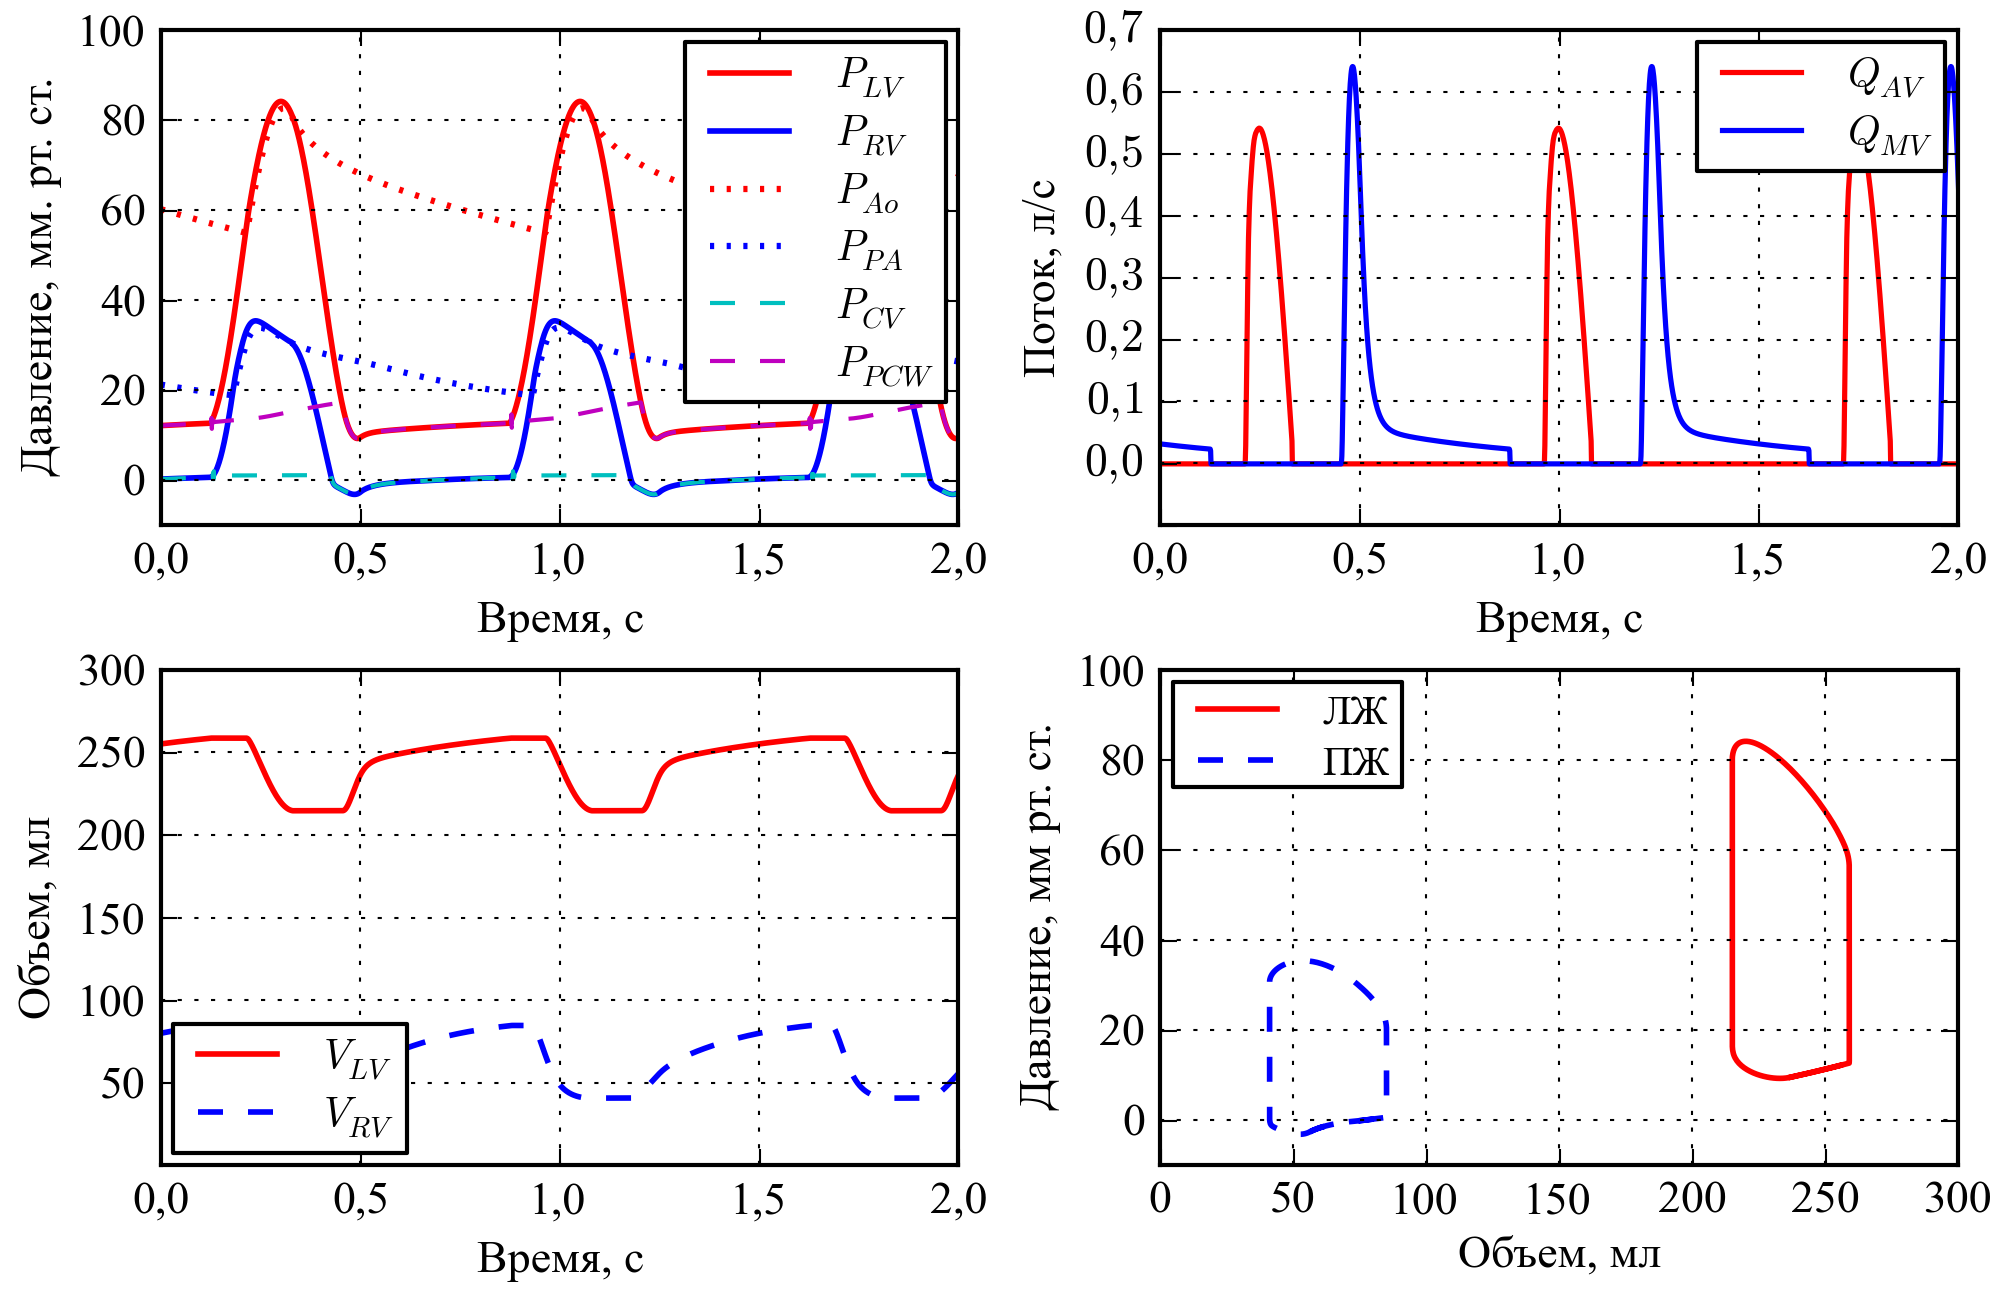
\includegraphics[width=1.0\linewidth]{../images/cvs_hemodynamics_pres}}
\caption{\scriptsize Гемодинамика в сердечной-\\сосудистой системе в условиях сердечной недостаточности; \tiny $P_{LV}$ -- давление в левом желудочке сердца, $P_{RV}$ -- давление в правом желудочке сердца, $P_{Ao}$ -- давление в аорте, $P_{PA}$ -- давление в легочной артерии, $P_{CV}$ -- центральное венозное давление, $P_{PCW}$ -- давление заклинивания в легочных капиллярах, $Q_{AV}$ и $Q_{MV}$ -- потоки через аортальный и митральный клапаны, $V_{LV}$ и $V_{RV}$ -- объемы левого и правого желудочков сердца}
\end{figure}

\end{minipage}
\vskip-2pt
\scriptsize Данные о гемодинамике в условиях сердечной недостаточности взяты из литературы \footnotemark[1]. Коэффициенты математической модели определены с помощью разработанной процедуры оптимизации на основе алгоритма Левенберга-Марквардта \footnotemark[2]. 

\vskip6pt
\footnotetext[1]{\tiny ~\textit{Cox L. G., Loerakker S., Rutten M. C. et al.} A Mathematical Model to Evaluate Control Strategies for Mechanical Circulatory Support \textcolor{pGray}{// Artificial Organs. 2009. Vol. 33, no. 8. P. 593-603.} }

\footnotetext[2]{\tiny ~\textit{Petukhov D. S., Telyshev D. V.} A mathematical model of the cardiovascular system of pediatric patients with congenital heart defect \textcolor{pGray}{// Biomedical Engineering. 2016. Vol. 50, no. 4. P. 229-232.} }

% \vskip6pt
% \footnotetext[3]{\tiny ~\textit{Петухов Д. С., Телышев Д. В.} Математическая модель сердечно-сосудистой системы педиатрических пациентов с врожденными пороками сердца \textcolor{pGray}{// Медицинская техника. 2016. № 4. С. 9--11.} }

% \footnotetext[2]{\scriptsize ~\textit{Martina J. R., Bovendeerd P. H., de Jonge N. et al.} Simulation of Changes in Myocardial Tissue Properties During Left Ventricular Assistance With a Rotary Blood Pump \textcolor{pGray}{// Artificial Organs. 2013. Vol. 37, no. 6. P. 531-540.} }

\end{frame}

% ------------------------------------------------------------------------------

\begin{frame}{Моделирование взаимодействия РНК и сердечно-сосудистой системы}

\begin{minipage}[ht]{0.34\textwidth}
\scriptsize

\begin{figure}
\center{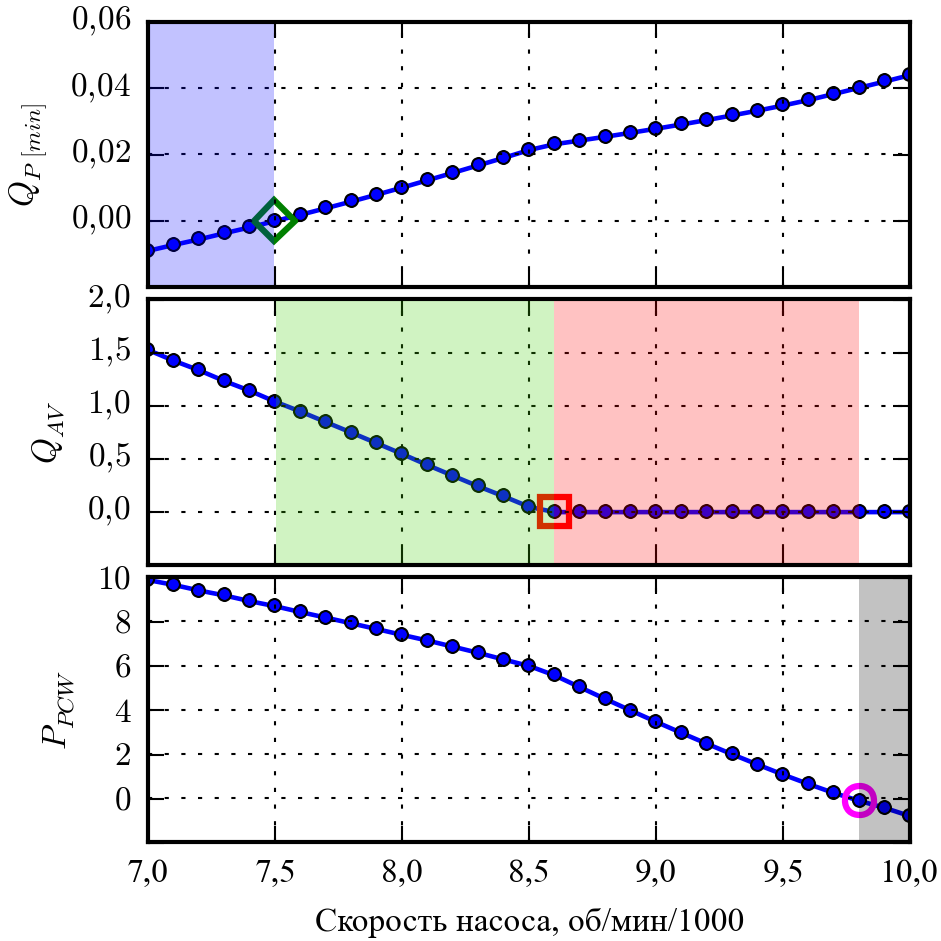
\includegraphics[width=1.0\linewidth]{../images/pumping_states_pres}}
\caption{\scriptsize Режимы работы насоса, определенные из гемодинамических зависимостей на модели сердечно-сосудистой системы; \\ \tiny $Q_{P[min]}$ -- минимальный расход насоса (л/с), $Q_{AV}$ -- поток через аортальный клапан (л/мин), $P_{PCW}$ -- давление заклинивания в легочных капиллярах (мм рт. ст.)}
\end{figure}

%\vskip-5pt
Определены режимы работы насоса -- обратное течение через насос, частичная и полная разгрузка желудочка и коллапс желудочка сердца. % \footnotemark[1].%$^, $\footnotemark[3]. 

\end{minipage}
\hfill
\begin{minipage}[ht]{0.64\textwidth}
\scriptsize

\vskip6pt
Предложены \underline{критерии оценки эффективности идентификации}:
\vskip-3pt
\begin{itemize}
 \item точность оценки расхода насоса $\delta(Q) \geq 90\%$, \vskip-5pt
 \item \vskip-3pt точность определения перехода между режимами работы насоса $\delta(PS) \geq 80\%$.
\end{itemize}

\vskip-3pt
\tiny Точность оценки расхода насоса вычисляется по формуле:

\vskip-4pt
\begin{equation}
	\delta(Q) = \left( 1 - (Q_M - Q_E)/Q_M \right) \cdot 100 \%,
\end{equation}

\vskip-3pt
где $Q_M$ -- расход насоса, измеренный датчиком, $Q_E$ -- расход насоса, оцененный с помощью математической модели. 

Точность определения перехода между режимами работы насоса вычисляется по формуле:

\vskip-8pt
\begin{equation}
	\delta(PS) = \left(1 - \frac{\lvert \omega_t - \omega_m \rvert}{\omega_{max} - \omega_{min}} \right) \cdot 100\%,
\end{equation}

\vskip-2pt
где $\omega_t$ -- скорость при переходе между режимами работы, определенная из гемодинамической зависимости, $\omega_m$ -- скорость при переходе между режимами работы, определенная с помощью производной, $\omega_{max}$ и $\omega_{min}$ -- верхняя и нижняя граница скорости насоса.

\vskip3pt
Разработан \emph{метод определения режимов работы насоса}, который заключается в анализе производных, найденных из математической модели идентификации, при различных скоростях насоса \footnotemark[1]. 

\vskip-11pt
\tiny
\setcounter{table}{0}
\begin{table}
\caption{\tiny Результаты расчета точности определения перехода между режимами работы насоса ($\delta(PS)$, \%) на математической модели сердечно-сосудистой системы в различных физиологических условиях при $\mu$ 3,6 сП}\vskip-5pt
\begin{tabular}{lrrr}
\toprule
 & Сократимость & ЧСС & Среднее\\
\midrule
$\delta(P_{BF}/P_{PA})$				& 89,3		&	88,0		& 88,6\\
$\delta(P_{PA}/P_{FA})$				& 98,0		& 98,0		& 98,0\\
%$\delta(P_{FA}/P_{PVC})$				& 92,0		& 89,3		& 90,6\\
$\delta(P_{FA}/P_{VC})$			& 84,0		& 81,3		& 82,6\\
\bottomrule
\end{tabular}
\end{table}

\end{minipage}

\vskip2pt

\footnotetext[1]{\tiny ~\textit{Petukhov D. S., Telyshev D. V.} Simulation of blood flow dynamics changes through implantable axial flow pump \textcolor{pGray}{// Biomedical Engineering. 2015. Vol. 48, no. 6. P. 336-340.} }

\end{frame}

% ------------------------------------------------------------------------------

\begin{frame}{Экспериментальное исследование Спутник}

\scriptsize
\begin{minipage}[ht]{0.49\textwidth}

Имплантируемые роторные насосы крови Спутник:

$\cdot$ Спутник 1~~~~~~~~~~~~~~~~~~~~~~~~~~~~~~~$\cdot$ Спутник 2

\includegraphics[scale=0.06]{../images/c1_s1}~~~~~~~~~~~~\includegraphics[scale=0.06]{../images/c1_s2}

\vskip5pt
Испытательный гидродинамический стенд \tiny (Институт Гельмгольца по биомедициской инженерии, г. Ахен, Германия) \vskip2pt

{~~~~~~~~~~~~~~~~\centering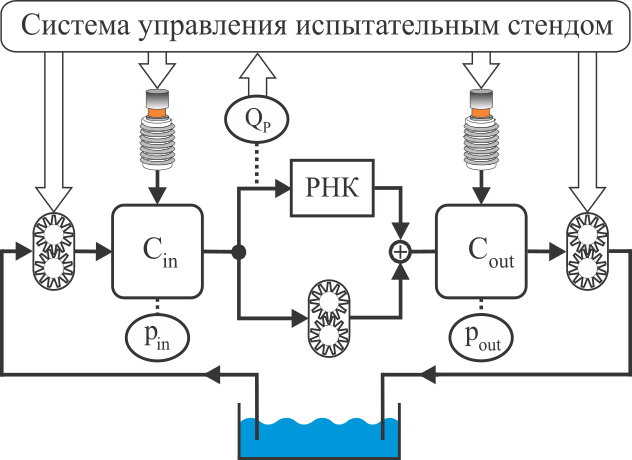
\includegraphics[scale=0.65]{../images/mcl_scheme_pres}}

\vskip5pt
\tiny Частота сердечных сокращений 80 уд/мин, вязкость жидкости в контуре 2,5 сП. Воспроизведены два состояния сердечно-сосудистой системы, соответствующие различным степеням сердечной недостаточности (contractilityFactor, cF): cF 0.5 и cF 0.25 \\ \vskip5pt

\vskip-5pt
{~~~~~~~~~~~~~~~~~~\centering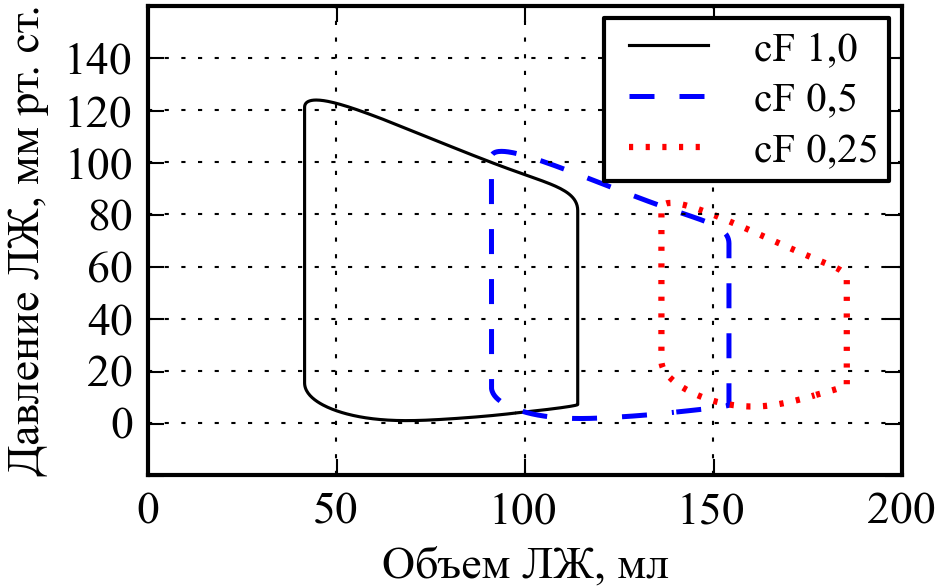
\includegraphics[scale=0.35]{../images/mcl_cF_pres}}

\end{minipage}
\hfill
\begin{minipage}[ht]{0.49\textwidth}
\scriptsize

\vskip3pt
Результаты экспериментального исследования: 
\vskip-14pt
\begin{figure}
  \center
  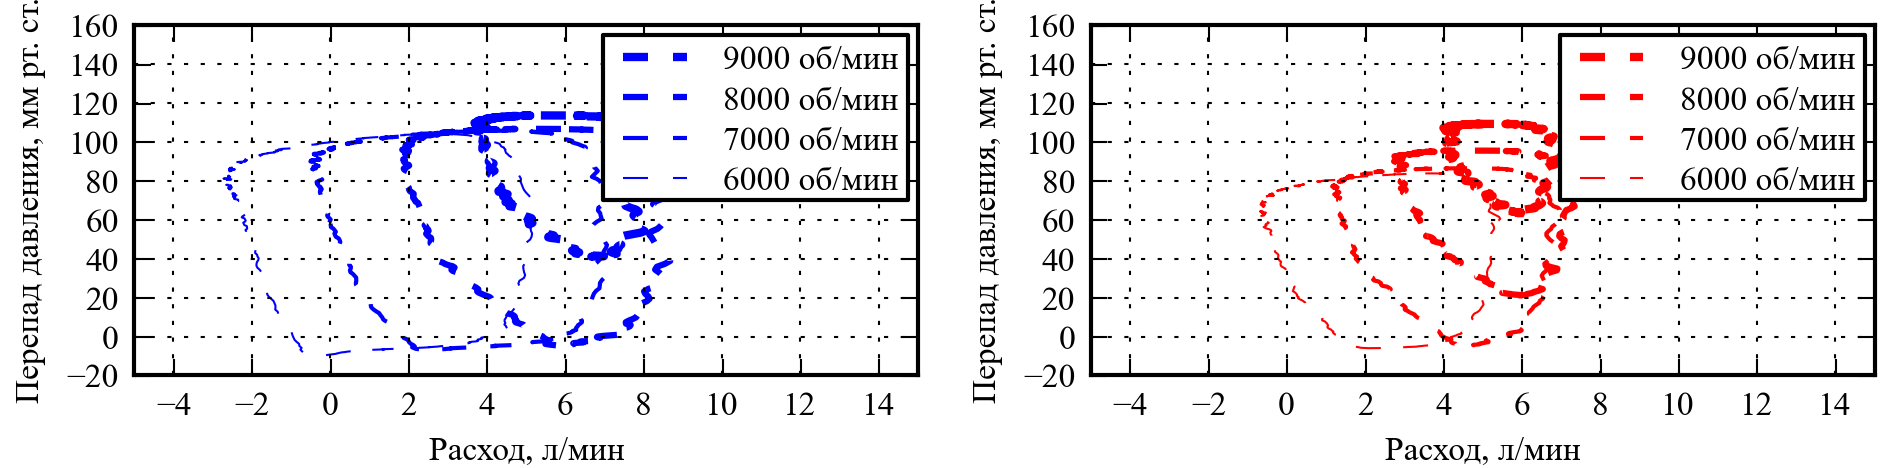
\includegraphics[scale=0.35]{../images/hq_s1_pres}
  \vskip-8pt\caption{\tiny Расходно-напорные характеристики Спутник 1} 
\end{figure}
\vskip-20pt
\begin{figure}
  \center
  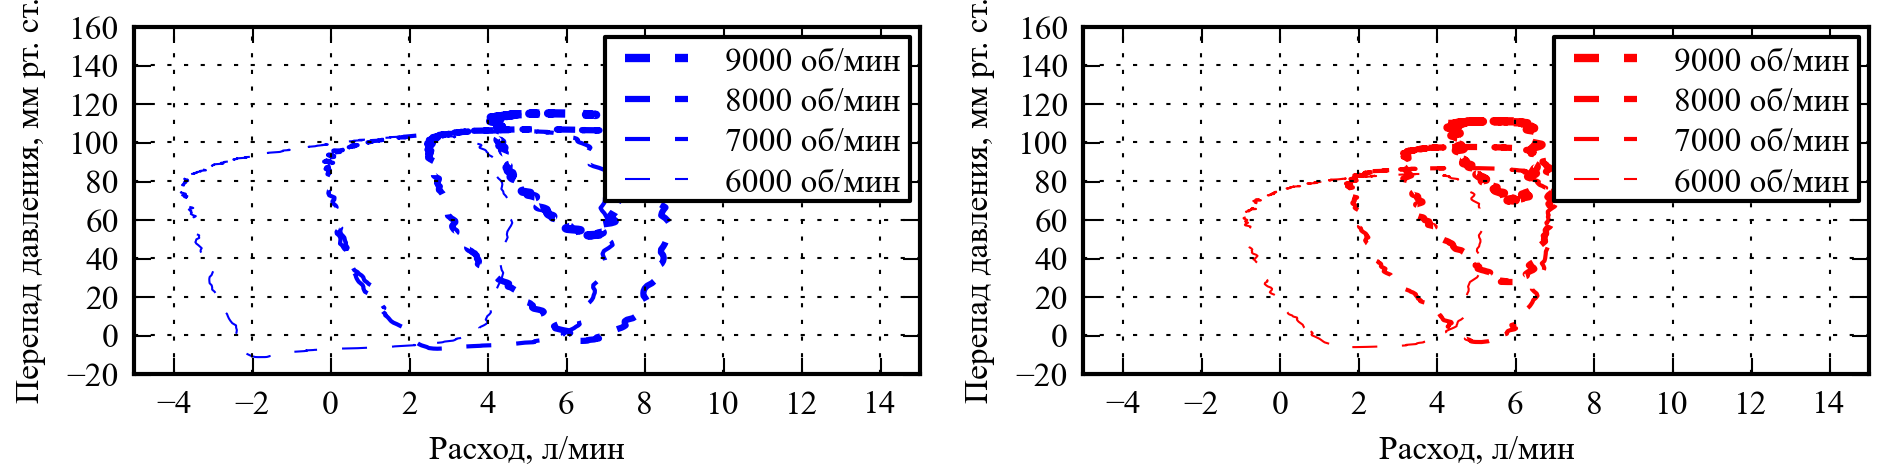
\includegraphics[scale=0.35]{../images/hq_s2_pres}
  \vskip-8pt\caption{\tiny Расходно-напорные характеристики Спутник 2} 
\end{figure}
\vskip-20pt
\begin{figure}
\center{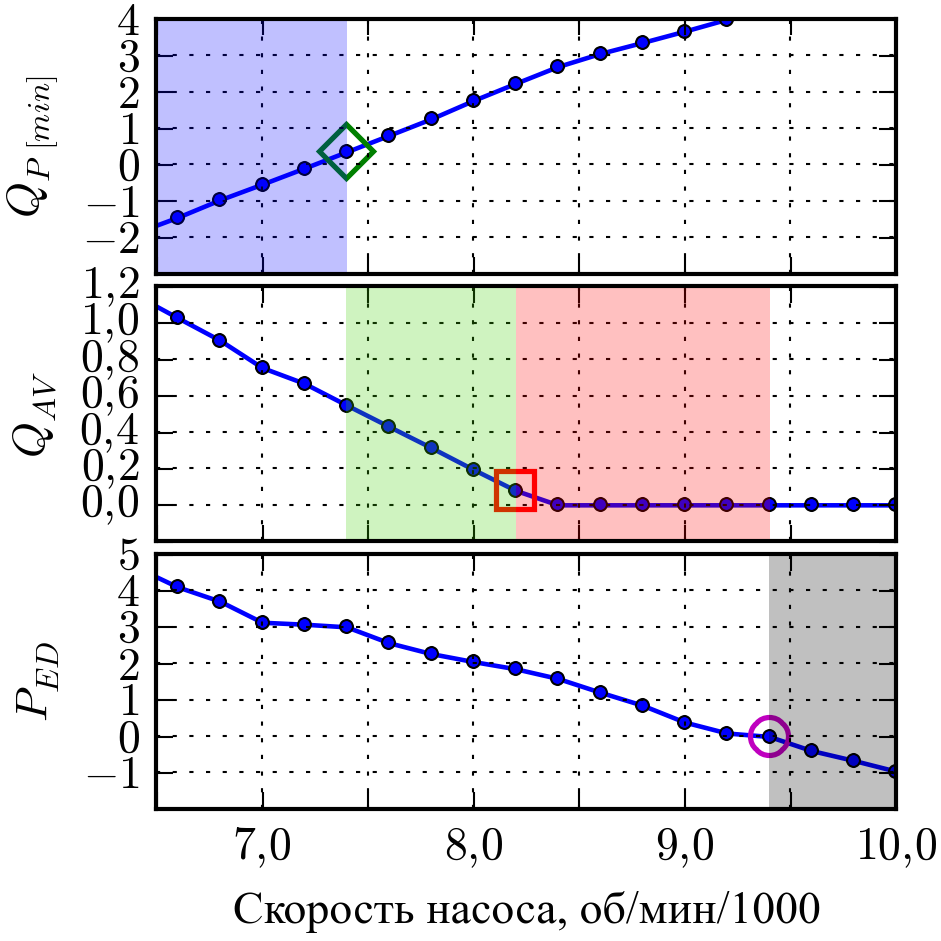
\includegraphics[width=0.515\linewidth]{../images/pumping_states_sputnik_1_pres}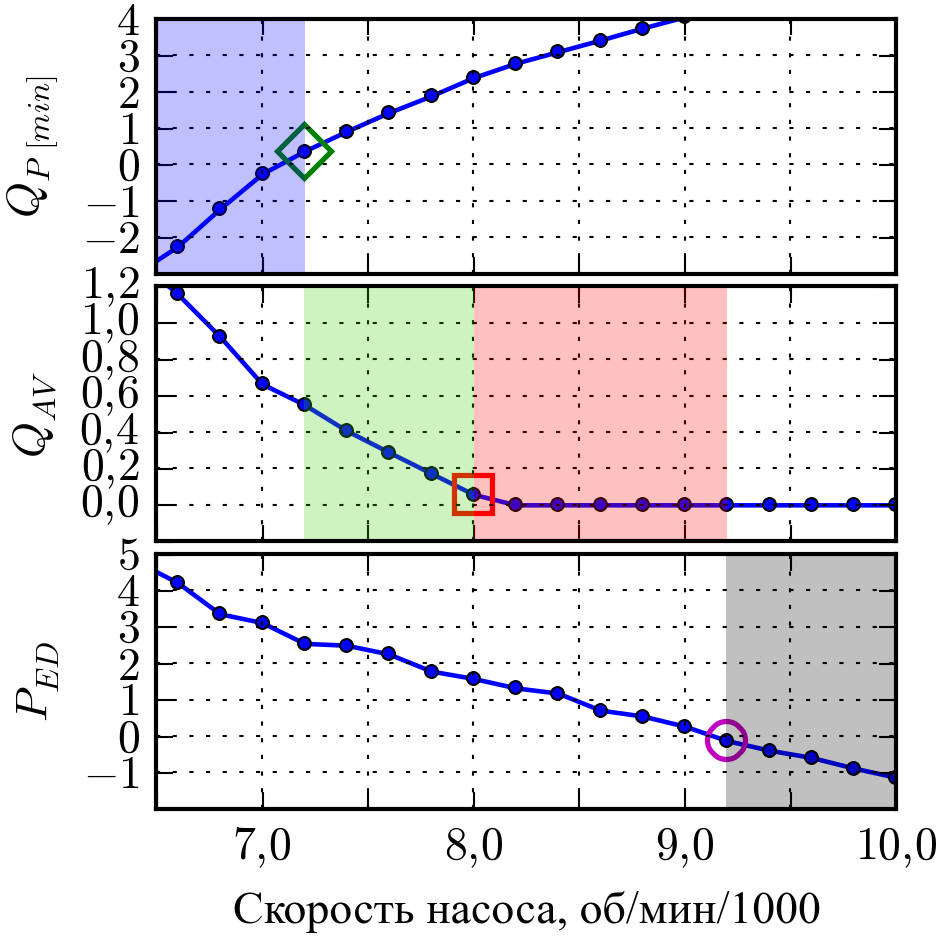
\includegraphics[width=0.515\linewidth]{../images/pumping_states_sputnik_2_pres}}
\vskip-8pt\caption{\tiny Режимы работы насоса, определенные из экспериментальных гемодинамических зависимостей:\\ Спутник 1 (слева) и Спутник 2 (справа); \\ $Q_{P[min]}$ -- минимальный расход насоса (л/мин), $Q_{AV}$ -- поток через аортальный клапан (л), $P_{ED}$ -- конечно-диастолическое давление в желудочке сердца (мм рт. ст.)}
\end{figure}

\vskip-4pt
\tiny \emph{Режим коллапса желудочка сердца} $P_{VC}$ определен как отрицательное конечно-диастолические давление в желудочке сердца.

\end{minipage}

\end{frame}

% ----------------------------------------------------------------------------------------------------------------------------------------------------------------
% ----------------------------------------------------------------------------------------------------------------------------------------------------------------

\begin{frame}{Проверка критериев оценки эффективности идентификации}

\scriptsize
Заданы следующие пороговые величины для критериев оценки эффективности идентификации:

\begin{itemize}
 \item \vskip-4pt средняя точность оценки расхода РНК $\delta(Q) \geq 90 \%$,
 \item \vskip1pt точность определения перехода между режимами работы РНК $\delta(PS) \geq 80 \%$.
\end{itemize} \small

\begin{minipage}[ht]{0.48\textwidth}
\vskip-14pt
\tiny Точность оценки расхода насоса вычисляется по формуле:

\vskip-3pt
\begin{equation}
	\delta(Q) = \left( 1 - (Q_M - Q_E)/Q_M \right) \cdot 100 \%,
\end{equation}

где $Q_M$ -- расход насоса, измеренный датчиком, $Q_E$ -- расход насоса, оцененный с помощью математической модели \footnotemark[1]. 

Исследованы два уравнения: разработанная математическая модель идентификации насоса HeartMate II и исходное уравнение для алгоритма идентификации \footnotemark[2].

Уравнение математической модели идентификации записывается в следующем виде:

\vskip-9pt
\begin{equation} \tag{3}
	L\frac{dQ}{dt} = aQ + b\omega^2 + cQ^2 + dQ^3 + eQ\omega^2 + fQ^2\omega + g - H.
\end{equation}
\vskip-2pt

Исходное уравнение для алгоритма идентификации записывается в следующем виде:

\vskip-4pt
\begin{equation} \tag{4}
	L\frac{dQ}{dt} = aQ + b\omega^2 + cH. %\text{\large \textcolor{red}{?}}
\end{equation}

\vskip0pt
Коэффициенты уравнений $L$, $a$ -- $g$ определены с помощью разработанной процедуры оптимизации на основе алгоритма дифференциальной эволюции. 

Исследованные уравнения позволяют оценить расход насоса и определить переходы между режимами работы насоса с точностью, которая 
\vskip-3pt
\large \bf \textcolor{red!70}{не соответствует критериям!}
\vskip-9pt
\end{minipage}
\hfill
\begin{minipage}[ht]{0.48\textwidth}

\tiny Точность определения перехода между режимами работы насоса вычисляется по формуле:

%\vskip-1pt
\begin{equation} \tag{2}
	\delta(PS) = \left(1 - \frac{\lvert \omega_t - \omega_m \rvert}{\omega_{max} - \omega_{min}} \right) \cdot 100\%,
\end{equation}

где $\omega_t$ -- скорость при переходе между режимами работы, определенная из гемодинамической зависимости, $\omega_m$ -- скорость при переходе между режимами работы, определенная с помощью производной, $\omega_{max}$ и $\omega_{min}$ -- верхняя и нижняя граница скорости насоса \footnotemark[1].

\vskip-10pt
\setcounter{table}{0}
\begin{table}
\caption{\scriptsize Точность оценки расхода насоса ($\delta(Q)$, \%) и точность определения перехода между режимами работы насоса ($\delta(PS)$, \%); \\ С1 -- Спутник 1, С2 -- Спутник 2}\vskip-3pt
\begin{tabular}{lrrrr}
\toprule
 & \multicolumn{2}{c}{Уравнение 1} & \multicolumn{2}{c}{Уравнение 2} \\
\midrule
    	& С1 & С2 & С1 & С2 \\
		\midrule
%		8600 & 99,9 & 95,1 & 98,1 & 95,1 \\
%		\midrule
		Среднее $\delta(Q)$ & 97,6 & \textcolor{red}{85,4} & \textcolor{red}{84,6}	&	\textcolor{red}{79,5} \\
\midrule
$\delta(P_{BF}/P_{PA})$		& 	91,7								&	95,8									&	$-$	& 91,7	\\
$\delta(P_{PA}/P_{FA})$		& 95,8								&	91,7									&	$-$	& $-$ \\
$\delta(P_{FA}/P_{VC})$		& 	\textcolor{red}{79,1}	& \textcolor{red}{70,8}		& $-$	& 91,7 \\

\bottomrule
\end{tabular}
\end{table}

\end{minipage}

\vskip-3pt

\footnotetext[1]{\tiny ~\textit{Petukhov D. S., Telyshev D. V.} An approach to the evaluation and control of a rotary blood pump using in vitro experimental results for two generations of LVAD Sputnik \textcolor{pGray}{// 24th Congress of the International Society for Rotary Blood Pumps. 2016. P. 70.} }

\footnotetext[2]{\tiny ~\textit{Petukhov D. S., Telyshev D. V., Selishchev S. V.} A method for identification of pumping states in an implantable rotary blood pump: experimental validation for the LVAD Sputnik \textcolor{pGray}{// 62nd ASAIO Annual Conference. 2016. P. 10.} }

\end{frame}

% ----------------------------------------------------------------------------------------------------------------------------------------------------------------
% ----------------------------------------------------------------------------------------------------------------------------------------------------------------

\begin{frame}{Результаты проверки критериев оценки эффективности идентификации}
\tiny

\begin{minipage}[ht]{0.56\textwidth} 

\underline{\textbf{Алгоритм структурно-параметрической идентификации для Спутник}}: \vskip2pt

Критерии оценки эффективности идентификации:
\begin{itemize}
 \item \vskip-3pt точность оценки расхода насоса $\delta(Q)$,
 \item \vskip-3pt точность определения перехода между режимами работы $\delta(PS)$.
\end{itemize}

\vskip4pt
\begin{tikzpicture}[node distance=0.8cm,overlay]
\tikzstyle{startstop} = [rectangle, rounded corners, minimum width=1.0cm, minimum height=0.6cm,text centered, draw=black, fill=gray!10,xshift=2.5cm,yshift=-5.2]
\tikzstyle{io} = [trapezium, trapezium left angle=70, trapezium right angle=110, minimum width=0.9cm, minimum height=0.6cm, text centered, draw=black, fill=gray!10]
\tikzstyle{process} = [rectangle, minimum width=1.1cm, minimum height=0.5cm, text centered, draw=black, fill=blue!30]
\tikzstyle{decision} = [diamond, minimum width=1.5cm, minimum height=0.65cm, text centered, draw=black, fill=gray!10]
\tikzstyle{arrow} = [thick,->,>=stealth]

\node (start) [startstop] {\parbox{3.1cm}{Задание пороговых величин для критериев оценки эффективности идентификации и исходного уравнения $y_i$ где $i$ -- номер итерации}};
\node (in1) [io, below of=start, yshift=-9.00] {\parbox{2.5cm}{Добавление к $y_i$ члена вида $k\omega^xH^yQ^z$ где $k$ -- коэффициент \\ $x$, $y$ и $z$ $\in [-2 .. 4]$ }};
\node (pro1) [process, below of=in1, yshift=-16.0] {\parbox{3.7cm}{Оптимизация коэффициентов $y_i + k\omega^xH^yQ^z$ для состояния cF 0,5 с использованием процедуры на основе алгоритма дифференциальной эволюции \\ Проверка соответствия критериям оценки эффективности идентификации $\delta(Q)$ и $\delta(PS)$}};
\node (dec1) [decision, below of=pro1, yshift=-0.5cm] {};% {\footnotesize\bf \parbox{1.5cm}{Соответствие \\ критериям}};
\node (dec2) [decision, below of=dec1, yshift=-0.08cm] {};
\node (out2a) [process, right of=dec2, xshift=1.7cm, minimum width=1.0cm, fill=yellow!40] {\parbox{2.0cm}{Задание $y_i + k\omega^xH^yQ^z$ исходным уравнением \\ $i = i + 1$ \\ $j = j + 1$}};
\node (out2b) [process, left of=dec1, xshift=-1.4cm, minimum width=1.0cm, fill=red!40] {\parbox{2.2cm}{Исключение $y_i + k\omega^xH^yQ^z$ \\ $j = j + 1$}};
\node (out2c) [startstop, below of=dec2, xshift=-2.5cm, yshift=0.15cm, minimum height=0.5cm, fill=green!40] {\parbox{2.5cm}{Окончательное $y_i + k\omega^xH^yQ^z$}};
% \node (stop) [startstop, below of=dec1, yshift=-1.1cm, fill=green!40, yshift=-0.1cm] {\small Окончательное $y_i + kx_j$};

\draw [arrow] (start) -- (in1);
\draw [arrow] (in1) -- (pro1);
\draw [arrow] (pro1) -- (dec1);
\draw [arrow] (dec2) -- node[anchor=south] {нет} (out2a);
\draw [arrow] (dec1) -- node[anchor=south] {~~~~~~нет} (out2b);
\draw [arrow] (dec1) -- node[anchor=west] {~~да} (dec2);
\draw [arrow] (dec2) -- node[anchor=west] {~~да} (out2c);
\draw [arrow] (out2a) |- ($(in1.east)+(0,-0.1)$);
\draw [arrow] (out2b) |- ($(in1.west)+(0.05,0.1)$);
%\draw [arrow] (out2b) ($(out2b.east)$)|- + (2.5,0) |- ($(in1.east)+(0.05,0.1)$); 
\draw (2.5, -3.95) node {$\delta(Q) | \delta(PS)$}; %  \\ $\delta(PS) \geq 85\%$
\draw (2.5, -4.85) node {$\delta(Q)~\&~\delta(PS)$}; %  \\ $\delta(PS) \geq 85\%$

\end{tikzpicture}

\tiny \vskip170pt
Построенные математические модели насосов исследованы на математической модели сердечно-сосудистой системы:

\begin{itemize}
 \item \vskip-4pt $\delta(P_{BF}/P_{PA})$ более 92\%,	 $\delta(P_{PA}/P_{FA})$ -- 100\%	\vskip-5pt
 \item \vskip-2pt невозможно определение $P_{VC}$ из-за постоянства скорости насоса.	\vskip-5pt
\end{itemize}

\end{minipage}
\hfill
\begin{minipage}[ht]{0.42\textwidth}

\vskip0pt
Структура исходного уравнения:

\vskip-4pt
\begin{equation}
LdQ/dt =  aQ + b\omega^2 + cH.
\end{equation}

\vskip-2pt
С использованием алгоритма структурно-параметрической идентификации построены математические модели, которые обеспечивают соответствие заданным пороговым величинам для критериев оценки эффективности идентификации.

\vskip5pt

Математическая модель Спутник 1:

\vskip-8pt
\begin{equation}
	L_1\frac{dQ}{dt} = a_1Q + b_1\omega^2 + c_1H + d_1HQ + e_1\omega^{-1} H^2 Q.
\end{equation}

Математическая модель Спутник 2:

\vskip-8pt
\begin{equation}
	L_2\frac{dQ}{dt} = a_2Q + b_2\omega^2 + c_2H + d_2HQ^3 + e_2\omega^{-1}Q.
\end{equation}

\vskip-18pt

\setcounter{table}{0}
\begin{table}
\caption{\tiny Точность оценки расхода насоса ($\delta(Q)$, \%) и точность определения перехода между режимами работы насоса ($\delta(PS)$, \%)}\vskip-9pt
\begin{tabular}{lrrrr}
\toprule
 & \multicolumn{2}{c}{Спутник 1} & \multicolumn{2}{c}{Спутник 2} \\
\midrule
    	 & cF 0,5 & cF 0,25 & cF 0,5 & cF 0,25 \\
		\midrule
		Среднее $\delta(Q)$ & 93,7 & 93,6 & 90,1 & 94,6 \\
		\midrule
$\delta(P_{BF}/P_{PA})$		& 91,7			&	91,7			& 100,0		& 100,0\\
$\delta(P_{PA}/P_{FA})$		& 100,0		&	100,0		& 100,0		& 100,0\\
$\delta(P_{FA}/P_{VC})$		& 	100,0		&	100,0		& 91,7			& 91,7 \\
\bottomrule
\end{tabular}
\end{table}

\vskip-2pt
\centering~~~~~~~\large \bf \textcolor{green!70}{Соответствие критериям!}

\end{minipage}

\end{frame}

% ----------------------------------------------------------------------------------------------------------------------------------------------------------------
% ----------------------------------------------------------------------------------------------------------------------------------------------------------------

\begin{frame}{Управление имплантируемым роторным насосом крови}
\scriptsize

В результате проведенного комплексного исследования взаимодействия математических моделей идентификации и сердечно-сосудистой системы разработан \underline{способ управления роторным насосом крови}. %\footnotemark[1]$^,$\footnotemark[2]

\begin{minipage}[ht]{0.49\textwidth}
\begin{figure}
\center{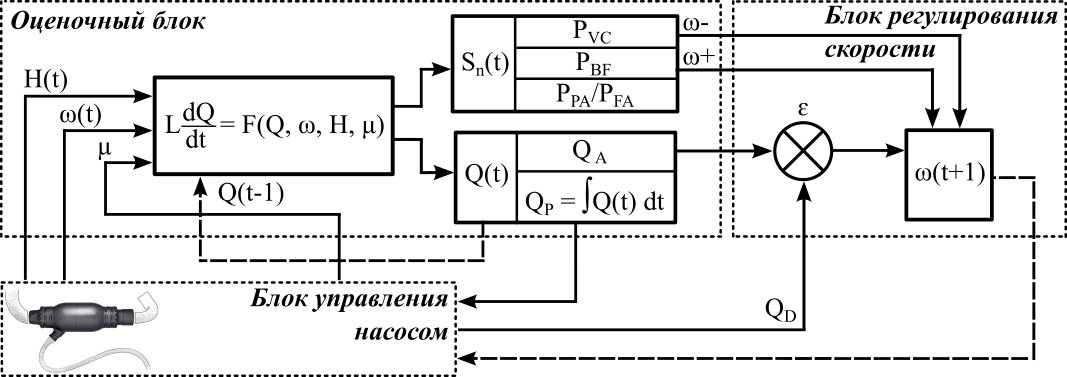
\includegraphics[width=0.99\linewidth]{../images/c3_control_algorithm}}
\caption{\scriptsize Обобщенная структура системы управления скоростью роторного насоса крови; \tiny \\$H$ -- перепад давления в насосе, $\omega$ -- скорость вращения ротора насоса, $\mu$ -- вязкость жидкости, $Q$ -- расход жидкости} % добавить расшифровку символов?
\end{figure}

\scriptsize \vskip-5pt
Для оценки расхода и определения режимов работы на основе известных $H$, $\omega$ и $\mu$ используется разработанная модель идентификации насоса HeartMate II:

\vskip-10pt
\begin{equation}
	\setcounter{equation}{1}
	L\frac{dQ}{dt} = aQ + b\omega^2 + cQ^2 + dQ^3 + eQ\omega^2 + fQ^2\omega + g - H.
\end{equation}

\end{minipage}
\hfill
\begin{minipage}[ht]{0.49\textwidth}
\vskip2pt
\begin{figure}
\center{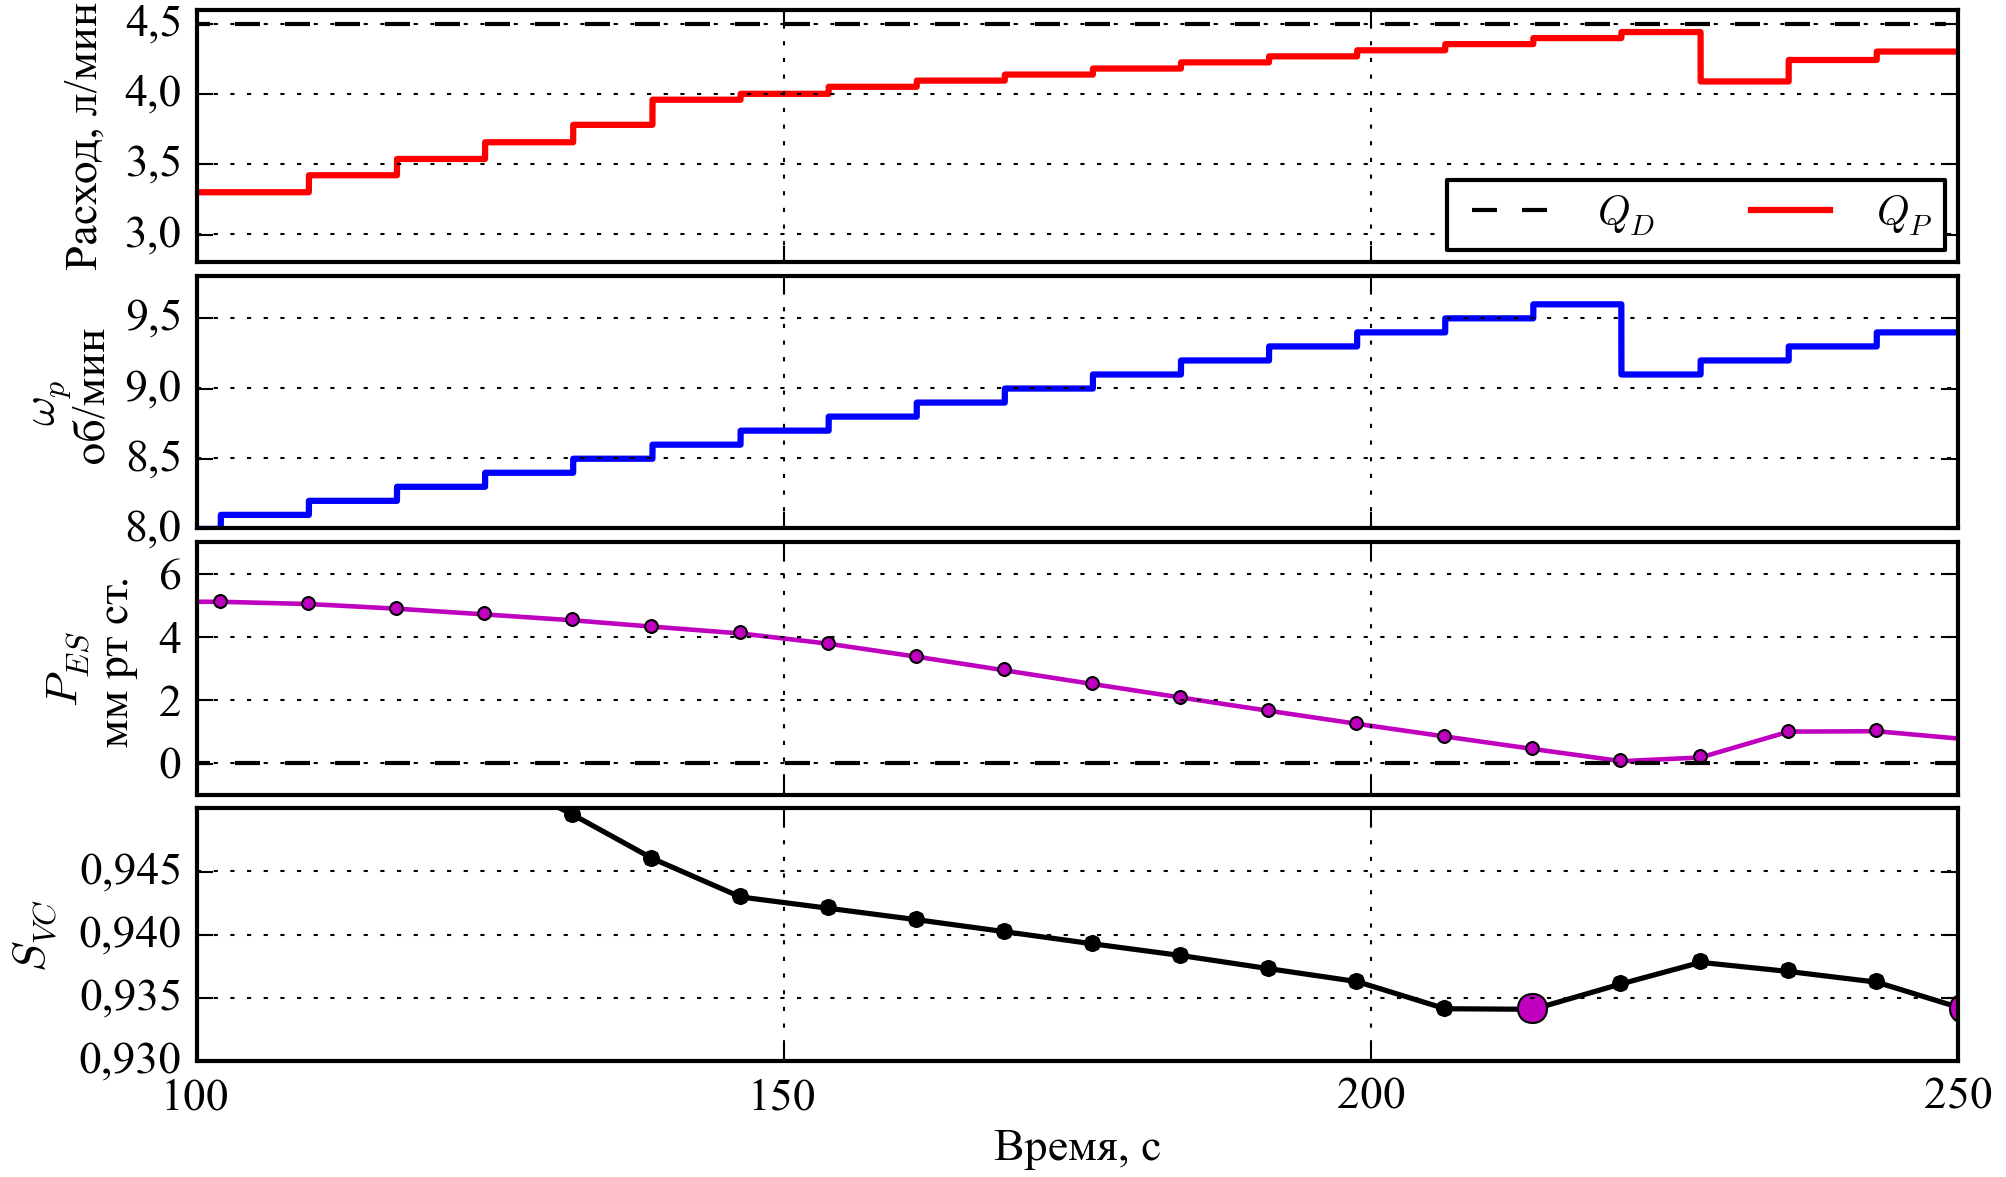
\includegraphics[width=0.99\linewidth]{../images/waveform_vc_pres}}
\vskip-6pt\caption{\tiny Пример управления скоростью роторного насоса крови $\omega_P$ с целью поддержания заданного уровня расхода $Q_D$ 4,5 л/мин и предотвращения режима коллапса желудочка сердца; $Q_P$ -- расход насоса, $P_{ES}$ -- конечно-систолическое давление в желудочке сердца, $S_{VC}$ -- индекс для определения $P_{VC}$ на основе производной $dQ/dt$} % добавить расшифровку символов?
\end{figure}

\end{minipage}

\vskip2pt
%Основной компонент схемы -- \emph{оценочный блок} -- позволяет оценивать расход и определять режимы работы с использованием математической модели идентификации РНК 

\vskip-3pt
Разработанный способ управления с использованием скорости вращения ротора в качестве управляемой переменной \footnotemark[1]$^-$\footnotemark[3] направлен на поддержание заданного уровня расхода насоса и предотвращение следующих нежелательных режимов работы насоса: обратное течение через насос, полная разгрузка желудочка сердца и коллапс желудочка сердца.

\vskip6pt

\footnotetext[1]{\tiny ~\textit{Petukhov D. S.} Simulation and control of the H-Q curves of the Sputnik portable ventricular assist device \textcolor{pGray}{// Biomedical Engineering. 2017. Vol. 50, no. 6. P. 429-432.} }

\footnotetext[2]{\tiny ~\textit{Petukhov D. S., Telyshev D. V., Selishchev S. V.} Control method of a rotary blood pump for a left ventricular assist device \textcolor{pGray}{// Sovremennye tehnologii v medicine 2016. Vol. 8, no. 1. P. 28-33.}}

\footnotetext[3]{\tiny ~\textit{Petukhov D. S., Telyshev D. V.} Design concept of patient-adaptive control method for a ventricular assist device \textcolor{pGray}{// 37th Annual International Conference of the IEEE Engineering in Medicine and Biology Society. 2015. P. 116.} }

% $\bf P_{BF}$ -- режим обратного течения через насос, $\bf P_{PA}$ -- режим частичной разгрузки желудочка сердца, $\bf P_{FA}$ -- режим полной разгрузки желудочка сердца, $\bf P_{PVC}$ -- режим частичного коллапса желудочка сердца, $\bf P_{FVC}$ -- режим полного коллапса желудочка сердца.

\end{frame}

% ----------------------------------------------------------------------------------------------------------------------------------------------------------------

\begin{frame}{Внедрение результатов диссертационной работы}

\begin{minipage}[ht]{0.46\textwidth}
\scriptsize
Результаты диссертационной работы:

\begin{itemize}
 \item использованы при реализации следующих проектов и исследований:
 \begin{itemize} \tiny
  \item проект Российского научного фонда \\ № 14-39-00044 <<Разработка адаптивной системы вспомогательного кровообращения с целью персонализации лечения острой формы сердечной недостаточности>> (2014 - 2016 гг.),
  \item прикладные научные исследования по теме <<Разработка аппарата длительного механического замещения функции сердца>> (RFMEFI57814X0057) (2014 - 2016 гг.),
  \item прикладные научные исследования и экспериментальные разработки по теме <<Миниатюризация имплантируемых насосов крови для их применения в педиатрической кардиохирургии>> \\ (RFMEFI58115X0014) (2015 - 2017 гг.).
 \end{itemize}
% \item внедрены в учебный процесс кафедры биомедицинских систем Национального исследовательского университета <<МИЭТ>> в рамках дисциплины <<Биомедицинская инженерия искусственных органов>>
\end{itemize}
\end{minipage}
\hfill
\begin{minipage}[ht]{0.52\textwidth}
\scriptsize \vskip-8pt
Акты о внедрении результатов диссертационной работы
\begin{figure}
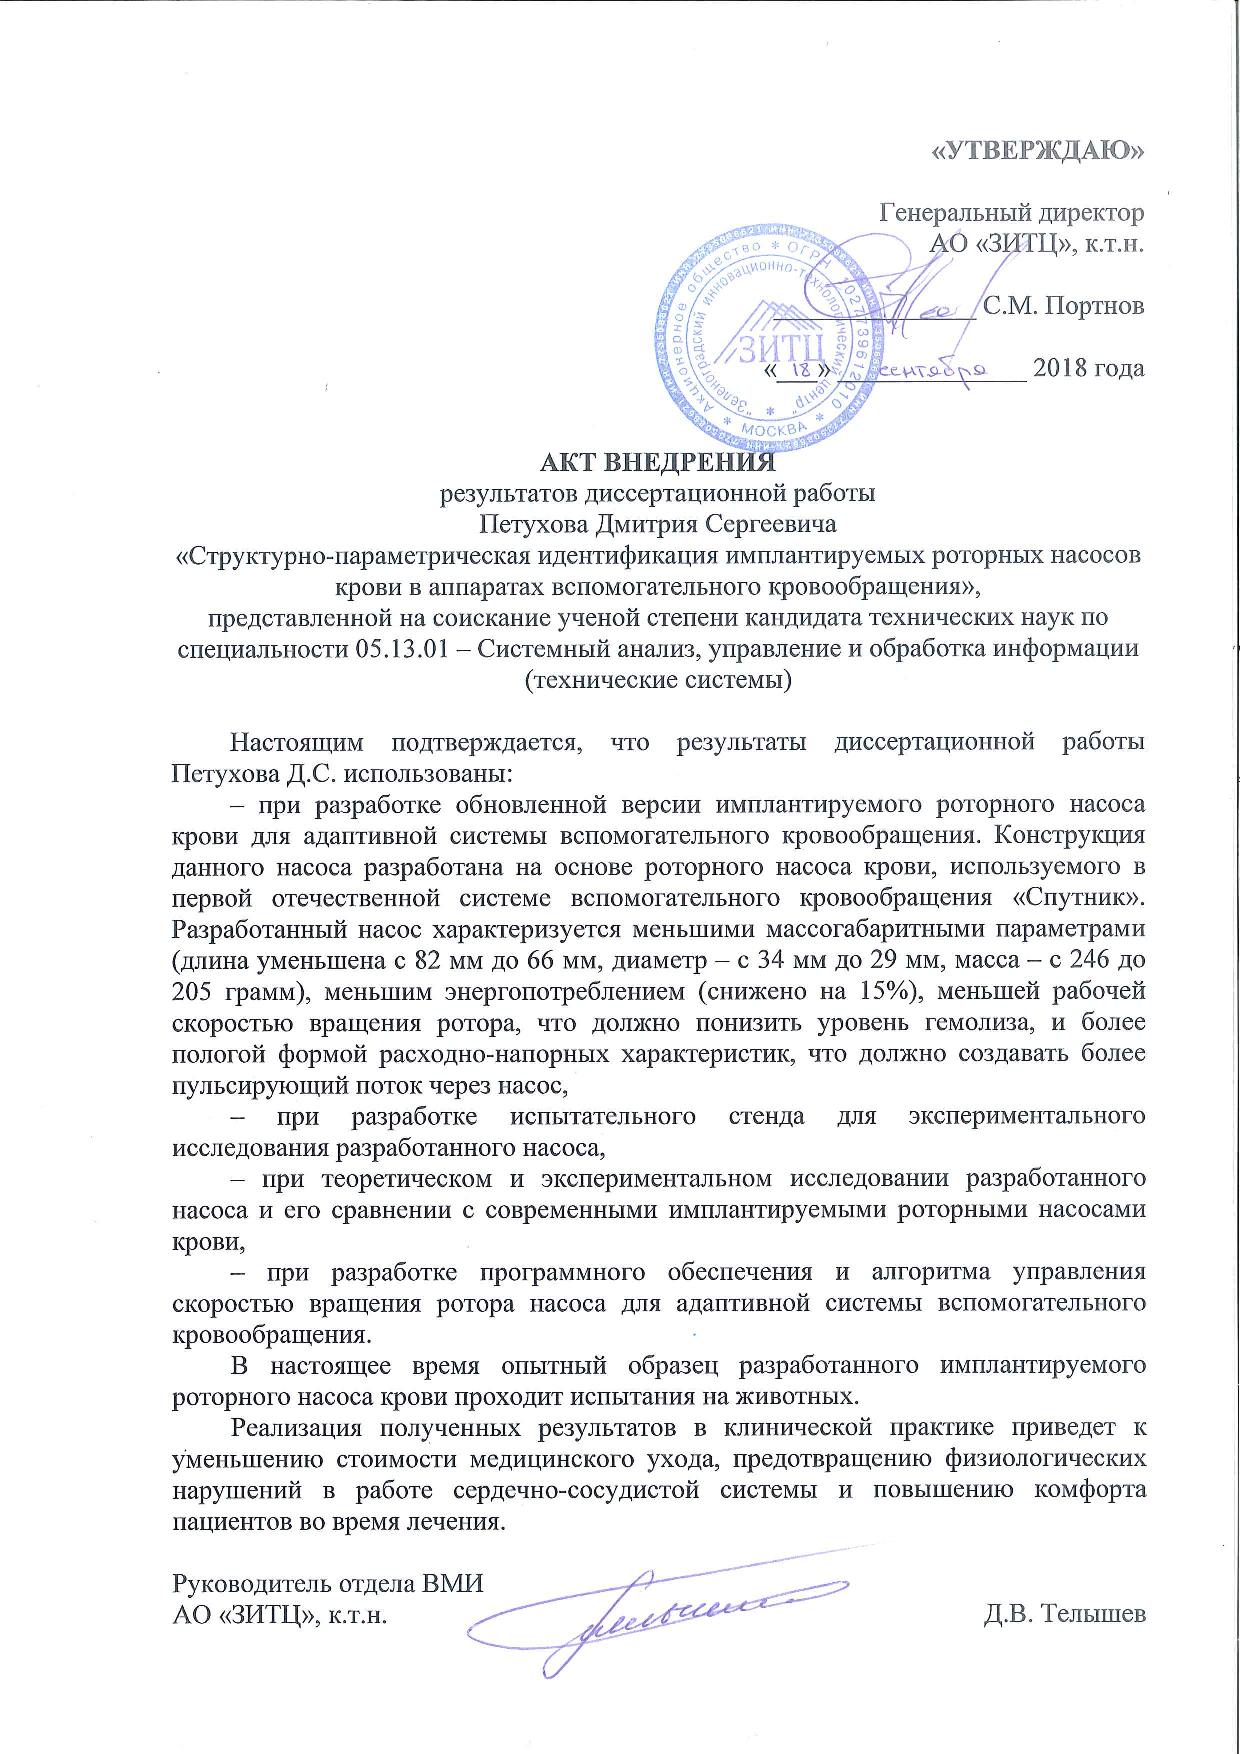
\includegraphics[width=0.75\linewidth,angle=-90,origin=c]{../images/act_1} 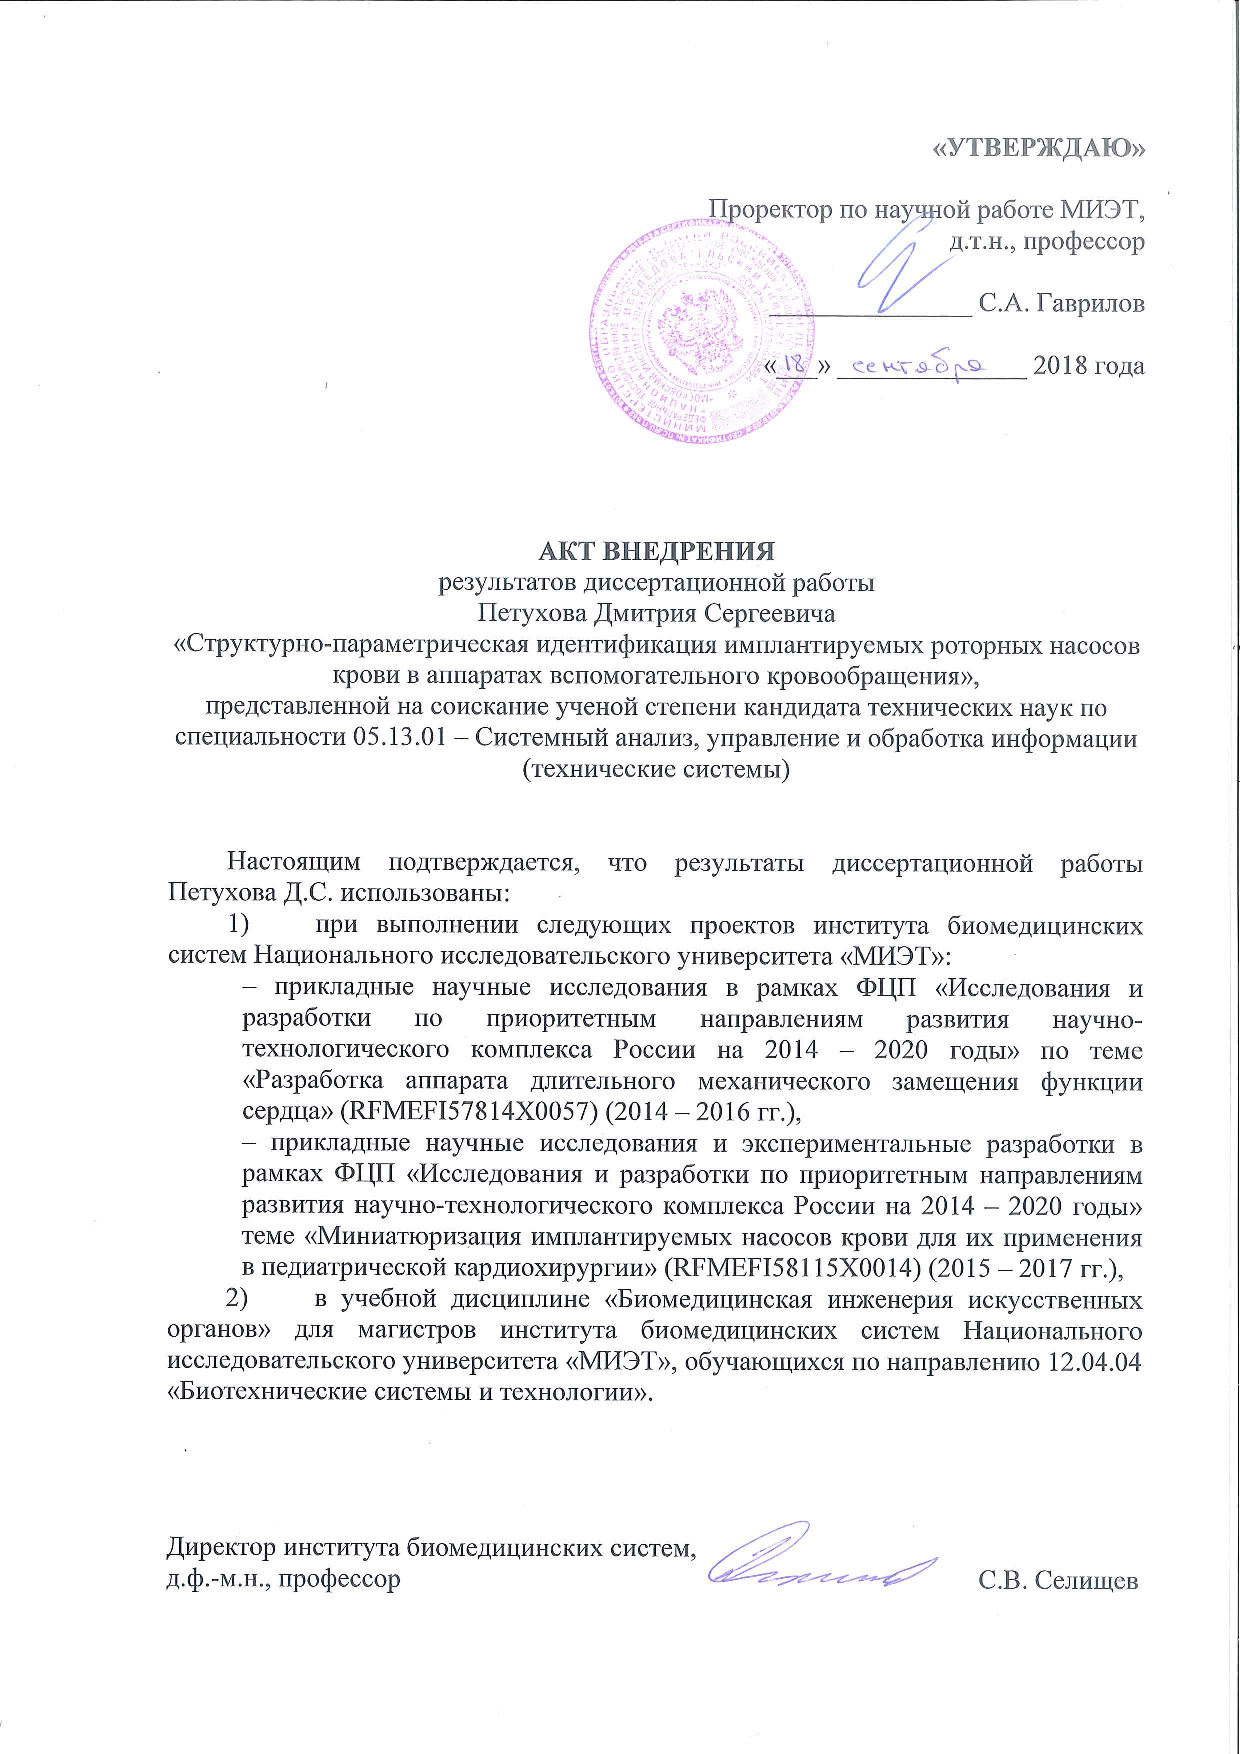
\includegraphics[width=0.75\linewidth,angle=-90,origin=c]{../images/act_2}
\end{figure}

\end{minipage}
\scriptsize
\begin{itemize}
 \item внедрены в учебный процесс института биомедицинских систем Национального исследовательского университета <<МИЭТ>> в рамках дисциплины <<Биомедицинская инженерия искусственных органов>> для магистров, обучающихся по направлению 12.04.04 <<Биотехнические системы и технологии>>
\end{itemize}
\end{frame}

% ----------------------------------------------------------------------------------------------------------------------------------------------------------------

\begin{frame}{Апробация диссертационной работы}
\footnotesize

Основные результаты работы были представлены на 18 всероссийских и международных конференциях:

\begin{itemize}
 \item 44th Annual ESAO and 7th IFAO Congress (г. Вена, Австрия, 2017),
 \item 2nd International Symposium <<Physics, Engineering and Technologies for Biomedicine>> \\(г. Москва, 2017),
 \item 20-23-я всероссийская конференция <<Микроэлектроника и информатика>> (г. Москва, 2013 -- 2016),
 \item 61-62nd ASAIO Annual Conference (г. Чикаго, США, 2015; г. Сан-Франциско, США, 2016),
 \item 24th Congress of the International Society for Rotary Blood Pumps (г. Мито, Япония, 2016),
 \item X-XI German-Russian Conference on Biomedical Engineering (г. Санкт-Петербург, 2014; \\г. Ахен, Германия, 2015),
 \item 42th Annual ESAO Congress (г. Лёвен, Бельгия, 2015),
 \item 37th Annual International Conference of the IEEE Engineering in Medicine and Biology Society (г. Милан, Италия, 2015),
 \item 16-я научно-техническая конференция <<МедТех>> (о. Кефалония, Греция, 2014),
 \item 11-я международная конференция <<Физика и радиоэлектроника в медицине и экологии>> (г. Суздаль, 2014),
 \item 6-я Троицкая конференция <<Медицинская физика и инновации в медицине>> (г. Троицк, 2014).
\end{itemize}

\end{frame}

% ----------------------------------------------------------------------------------------------------------------------------------------------------------------

\begin{frame}
\frametitle{Список основных публикаций}

\scriptsize

Основные результаты работы были опубликованы в 11 рецензируемых научных изданиях, входящих в перечень Высшей аттестационной комиссии при Министерстве образования и науки Российской Федерации: 

\begin{enumerate}%[leftmargin=25pt, itemsep=12pt] %[leftmargin=2em, itemsep=2em]
  \item Петухов Д. С., Телышев Д. В. Исследование роторного насоса для поддержки кровообращения правого желудочка сердца при механической поддержке кровообращения обоих желудочков сердца // Медицинская техника. 2017. № 1. С. 24--26.
  \item Петухов Д. С. Моделирование и управление расходно-напорными характеристиками имплантируемого насоса крови АВК-Н <<Спутник>> // Медицинская техника. 2016. № 6. С. 52--55.
  \item Петухов Д. С., Телышев Д. В. Математическая модель сердечно-сосудистой системы педиатрических пациентов с врожденными пороками сердца // Медицинская техника. 2016. № 4. С. 9--11.
  \item Петухов Д. С., Телышев Д. В. Алгоритмы управления роторными аппаратами вспомогательного кровообращения // Медицинская техника. 2016. № 3. С. 8--11.
  \item Петухов Д. С., Телышев Д. В., Селищев С. В. Метод управления роторным насосом крови для системы вспомогательного кровообращения левого желудочка сердца // Современные технологии в медицине. 2016. Т. 8, № 1. С. 28--33.
  \item Петухов Д. С., Телышев Д. В. Исследование чувствительности роторного насоса крови <<Спутник>> к преднагрузке и постнагрузке // Медицинская техника. 2015. № 6. С. 27--30.
  \item Петухов Д. С., Селищев С. В., Телышев Д. В. Перспективы развития технологий полной замены функции сердца с помощью механических систем
поддержки кровообращения // Медицинская техника. 2015. № 5. С. 5--8.
  \item Петухов Д. С., Селищев С. В., Телышев Д. В. Полностью искусственное сердце: современное состояние // Медицинская техника. 2015. № 4. С. 1--4.
  \item Петухов Д. С., Телышев Д. В. Моделирование изменений в динамике течения крови через имплантируемый осевой насос // Медицинская техника. 2014. № 6. С. 44--47.
  \item Петухов Д. С., Селищев С. В., Телышев Д. В. Развитие аппаратов вспомогательного кровообращения левого желудочка сердца как наиболее эффективный способ лечения острой сердечной недостаточности // Медицинская техника. 2014. № 4. С. 37--39.
  \item Петухов Д. С., Селищев С. В. Оценка изменений в работе правого желудочка сердца при наличии аппарата вспомогательного кровообращения левого желудочка сердца // Медицинская техника. 2014. № 4. С. 28--32.
\end{enumerate}

\end{frame}

% ----------------------------------------------------------------------------------------------------------------------------------------------------------------

\begin{frame}{Основные результаты и выводы}
%\small
%\scriptsize
\scriptsize
%% Согласно ГОСТ Р 7.0.11-2011:
%% 5.3.3 В заключении диссертации излагают итоги выполненного исследования, рекомендации, перспективы дальнейшей разработки темы.
%% 9.2.3 В заключении автореферата диссертации излагают итоги данного исследования, рекомендации и перспективы дальнейшей разработки темы.
% \begin{enumerate}
%   \item Сформулированы основные требования к системе управления имплантируемым роторным насосом крови: точная оценка расхода РНК на основе доступных параметров насоса, поддержание требуемого уровня расхода в различных физиологических условиях либо обеспечение физиологического потока через насос, соответствующего потребностям организма, и предотвращение неблагоприятных состояний в сердечно-сосудистой системе, обусловленных спецификой работы роторного насоса;
%   \item Разработан метод косвенной оценки потока через имплантируемый роторный насос крови с учетом инерционных и вязкостных свойств крови;  
%   \item Разработан метод определения режимов работы имплантируемого роторного насоса крови с целью управления неблагоприятными состояниями в сердечно-сосудистой системе; он позволяет идентифицировать следующие режимы работы: обратное течение крови через насос, частичная разгрузка желудочка с периодически открывающимся аортальным клапаном, полная разгрузка желудочка с постоянно закрытым аортальным клапаном, частичный и полный коллапс желудочка во время сердечного цикла;
%   \item На базе разработанных методов предложен алгоритм управления имплантируемым роторным насосом крови, который удовлетворяет основным требованиям к современной системе управления для аппаратов вспомогательного кровообращения, кроме обеспечения физиологического потока через насос;
%   \item Разработанный метод определения режимов работы имплантируемого роторного насоса крови успешно проверен с использованием результатов испытаний двух поколений РНК, используемых в первом российском коммерческом аппарате вспомогательного кровообращения <<Спутник>> на гидродинамическом стенде в динамических условиях.
% \end{enumerate}

\begin{enumerate}

    \item Разработана математическая модель сердечно-сосудистой системы, которая позволила исследовать взаимодействие имплантируемого роторного насоса крови и сердечно-сосудистой системы в условиях сердечной недостаточности. 
	\item Разработан алгоритм структурно-параметрической идентификации, который позволил построить математические модели имплантируемых роторных насосов крови на основе их расходно-напорных характеристик в соответствии с критериями оценки эффективности идентификации. 
	\item Проведено исследование взаимодействия имплантируемого роторного насоса крови и сердечно-сосудистой системы методами математического моделирования. \\В результате исследования разработаны метод определения режимов работы роторного насоса крови и способ управления роторным насосом крови, который позволяет поддерживать заданный уровень расхода насоса и предотвращать нежелательные режимы работы насоса, а также предложены следующие критерии, которые позволяют оценить эффективность идентификации для управления имплантируемым роторным насосом крови: точность оценки расхода насоса и точность определения перехода между режимами работы насоса. 
	\item Проведено исследование взаимодействия имплантируемого роторного насоса крови и сердечно-сосудистой системы с использованием экспериментальных данных для роторных насосов крови Спутник, полученных в испытательном гидродинамическом стенде. При этом для критериев оценки эффективности идентификации заданы следующие пороговые величины: средняя точность оценки расхода насоса не менее 90\% и точность определения переходов между режимами работы насоса не менее 80\%. \\В результате исследования с использованием алгоритма структурно-параметрической идентификации и в соответствии с критериями оценки эффективности идентификации построены математические модели имплантируемых роторных насосов крови, которые обеспечивают среднюю точность оценки расхода насоса не менее 90\% и точность определения переходов между режимами работы насоса более 91\%.

%идентификация исследованных насосов с использованием разработанного алгоритма и следующих пороговых величин для критериев оценки эффективности: средняя точность оценки расхода насоса не менее 90\% и точность определения переходов между режимами работы насоса не менее 85\%. Построенные математические модели, которые обеспечивают соответствие заданным пороговым величинам для критериев оценки эффективности со средней точностью оценки расхода насоса не менее 90\% и точностью определения переходов между режимами работы насоса более 91\%.  \\

%На основе проведенного исследования в алгоритм идентификации внесены изменения, которые позволяют осуществлять поиск математической модели согласно пороговым величинам для критериев оценки эффективности. Описанные изменения позволили построить математические модели двух насосов

%   \item Разработана математическая модель роторного насоса крови с целью косвенной оценки потока через насос, учитывающая инерционные и вязкостные эффекты крови.
%   \item Разработан метод определения режимов работы роторного насоса крови на основе его математической модели, который продемонстрировал точность не менее 80 \% при тестировании на модели сердечно-сосудистой системы.
%   \item Разработан алгоритм управления роторным насосом крови, который удовлетворяет основным требованиям по регулированию работы насоса для аппаратов вспомогательного кровообращения, используемых в клинической практике.
%   \item Предложен алгоритм разработки математической модели роторного насоса крови с использованием результатов испытаний роторных насосов в динамических условиях, который обеспечил среднюю точность оценки расхода насоса не менее 90 \%.
%   \item Разработанный метод определения режимов работы роторного насоса крови проверен с использованием результатов испытаний двух поколений роторных насосов на гидродинамическом стенде в двух состояниях, соответствующих различным степеням сердечной недостаточности, продемонстрировав точность не менее 90 \%.
\end{enumerate}

% Предложенный в данной работе метод оценки потока через роторный насос крови является косвенным, т.\:е. вычисляет поток на основе доступных параметров насоса с некоторой точностью. В данной работе в качестве входных параметров модели используются перепад давления в насосе, его скорости и величина вязкости крови. В реальных условиях после имплантации РНК постоянное неинвазивное отслеживание перепада давления не представляется возможным, поэтому переход к собственным параметрам насоса, таким как электрический ток двигателя, скорость вращения или противо-ЭДС, остается основной задачей на ближайшее будущее. Предполагается, что возможное использование датчика расхода позволит в реальном времени рассчитывать поправочный коэффициент в виде величины вязкости крови, что также будет являться дополнительным диагностическим параметром. 
% 
% Разработанный метод определения режимов работы роторного насоса крови позволяет определить неблагоприятные состояния в сердечно-сосудистой системе, связанные с обратным течением крови через насос или коллапсом желудочком сердца, включая закрытое состояние аортального клапана при работающем РНК, что в долгосрочной перспективе позволит сохранить его функциональность, и реализовать новые стратегии лечения в том числе направленные на восстановление миокарда. 
% 
% Предложенный метод также генерирует различные варианты сигналов, описывающих динамику течения крови через насос и изменяющихся согласованно с изменениями этой динамики, за счет множества производных, которые можно получить из математической модели РНК. Это позволяет расширить возможности алгоритмов, основанных на анализе временных диаграмм сигналов насоса.
% 
% Данный метод был успешно протестирован на математической модели сердечно-сосудистой система и на гидродинамическом стенде в динамических условиях. При этом установлено, что он универсален и может быть использован для любых существующих роторных насосов крови. Одно из возможных его применений заключается в использовании в качестве средства неинвазивной диагностики сердечно-сосудистой системы при наличии АВК. Тем не менее, необходимыми являются испытания на животных и результаты клинических наблюдений за пациентами.
% 
% %В данной работе было показано, что такой подход обладает универсальностью и может быть использован для любых существующих роторных насосов крови. Он также реализует возможность использования роторного насоса в качестве средства диагностики и представляет собой основу для систем адаптивного управления роторными насосами крови в рамках существующей технологии. 
% 
% Предложенный алгоритм управления роторным насосом крови не реализует возможность физиологического управления роторным насос, т.\:е. не позволяет обеспечить расход насоса, соответствующий физиологическим потребностям организма. Но справедливости ради стоит отметить, что ни один из доступных в клинической практике АВК также не обладает такой возможностью. Реализация такой опции в коммерческой системе управления остается делом будущего.
% 
% Также следует отметить, что необходимым вариантом тестирования алгоритма управления, который не был рассмотрен в данной работе, является состояние сердечно-сосудистой системы под физической нагрузкой.
% 
% % в рамках выбранного применения АВК, которая будет заключаться в поддержании определенного режима работы РНК и, соответственно, обеспечении определенного физиологического состояния сердечно-сосудистой системы. 
% % 
% % Мы также осознаем, что в реальных динамических условиях после имплантации насоса постоянное отслеживание давления не представляется возможным, поэтому рассчитываем перейти к собственным параметрам насоса, таким как электрический ток, скорость вращения или противо-ЭДС.


\end{frame}

\end{document} 